%%%%%%%%%%%%%%%%%%%%%%%%%%%%%%%%%%%%%%%%%%%%%%%%%%%%%%%%%%%%%%
% Beamer Presentation
% LaTeX Template
% Version 1.0 (10/11/12)
%
% This template has been downloaded from:
% http://www.LaTeXTemplates.com
%
% License:
% CC BY-NC-SA 3.0 (http://creativecommons.org/licenses/by-nc-sa/3.0/)
%
%%%%%%%%%%%%%%%%%%%%%%%%%%%%%%%%%%%%%%%%%%%%%%%%%%%%%%%%%%%%%%

\documentclass{beamer}

\mode<presentation> {

\usetheme{Madrid}

}
\usepackage{graphicx} % Allows including images
\usepackage{booktabs} 

%-------------------------------------------------------------
%	TITLE PAGE
%-------------------------------------------------------------

\title[Course 62444]{Course 62444\\"Data Visualization and Analysis - Project"\\
%using Python/Spyder/Jupyter Notebook/\\ Google CoLab,\\ R/RStudio/RStudio.Cloud \&\\
%\LaTeX Beamer.
} 

\author{Bashar Khaled Bdewi}% Your name



\institute[DTU] % Your institution as it will appear on the bottom of every slide, may be shorthand to save space
{
\medskip
\textit{s183356@student.dtu.dk} 
}
\date{\today} 




%-------------------------------------------------------------

\begin{document}
\begin{frame}
\titlepage % Print the title page as the first slide
\end{frame}

\begin{frame}
\frametitle{The final report} % Table of contents slide, comment this block out to remove it
\tableofcontents
\end{frame}



\section{Seminar 1: Python/R and LATEX Tools and Platforms Review} 
%-------------------------------------------------------------
\begin{frame}
\frametitle{Seminar 1 - Table of Contents}
\begin{enumerate}
\item \textbf{R/RStudio} enviroment\newline
\footnotesize The examples are from \cite{Kabacoff2020}\newline

\item \textbf{Python}/Spyder/ Jupyter Notebook enviroment\newline
\footnotesize The examples are from \cite{VanderPlas2016}\newline

\item \textbf{The} \textbf{\LaTeX2e} Beamer Class \newline
\footnotesize\  Overleaf is used in this project.\newline

\item The folder structure
\end{enumerate}
\end{frame}



%-------------------------------------------------------------
%	PRESENTATION SLIDES
%-------------------------------------------------------------


% ##========================================================##
% ##                                                        ##
% ##                 Seminar 1                              ##
% ##                                                        ##
% ##========================================================##

\subsection{Verifying R/RStudio }
%-------------------------------------------------------------
\begin{frame}
\frametitle{Verifying R/RStudio}
Verifying the R/RStudio environment using examples from \footnotesize\cite{Kabacoff2020}.\newline

We nedd to  get current working directory :
\[ \text {Session} \rightarrow \text{Set Working Directory} \rightarrow \text{  62444\_PyR directory} \]

"salaries.csv" dataset.\newline

Reading the dataset:\\
Salaries \textless{- read\_csv ("salaries.csv")}
\end{frame}

%-------------------------------------------------------------
\begin{frame}[fragile] % Need to use the fragile option when verbatim is used in the slide
\frametitle{Verifying Rstudio: ggplot...Stacked bar plot}
\begin{example}[]
\begin{verbatim}
install.packages("ggplot2")
library(ggplot2)
# import data
url <- "https://bit.ly/3bsMwsS"
Salaries <- read.csv(url)
# review data
str(Salaries)
summary(Salaries)

# stacked bar plot
ggplot(data=Salaries, aes(x=rank, fill=sex)) + 
  geom_bar()
\end{verbatim}
\end{example}
\end{frame}
%-------------------------------------------------------------
\begin{frame}
\frametitle{Verifying Rstudio: ggplot...Stacked bar plot}
\begin{figure}
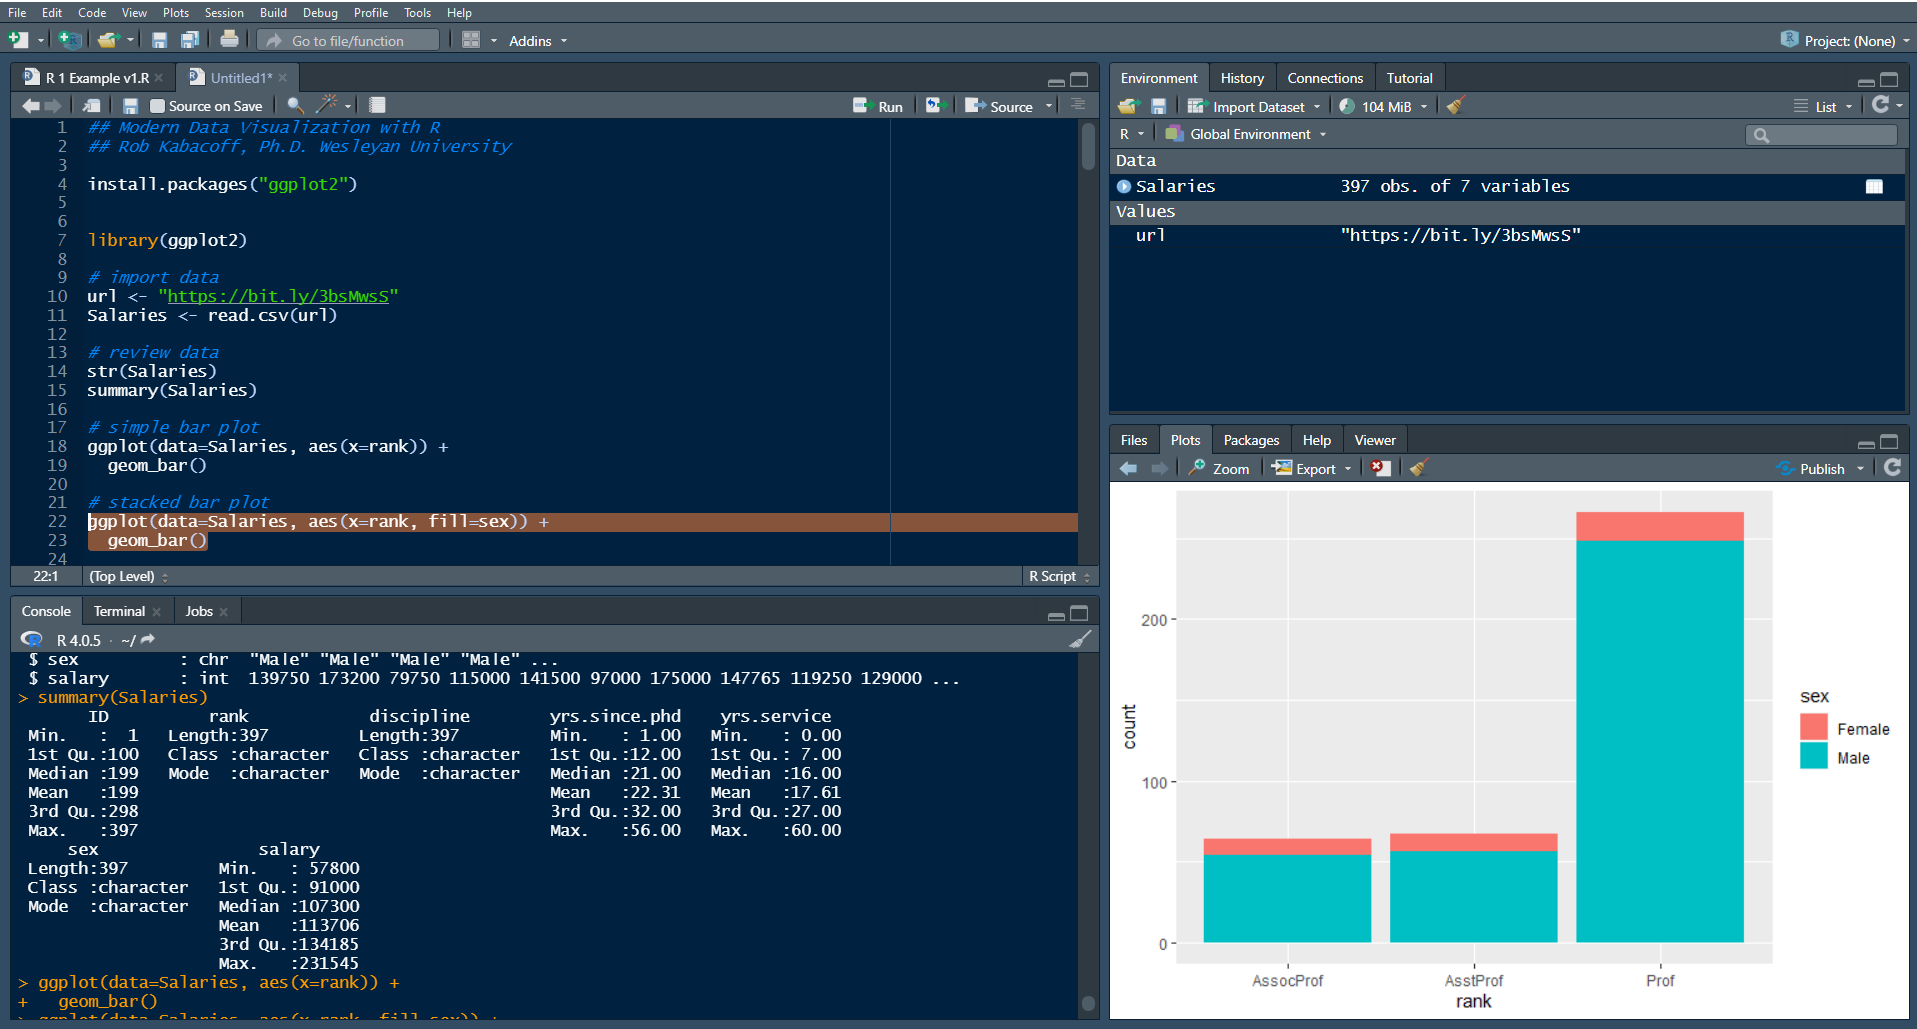
\includegraphics[width=1\linewidth]{Seminar_1_images/R.PNG}
\end{figure}
\end{frame}
%-------------------------------------------------------------
\subsection{Verifying python spyder }
%-------------------------------------------------------------
\begin{frame}[fragile] % Need to use the fragile option when verbatim is used in the slide
\frametitle{Verifying python spyder: Matplotlib...A simple histogram}
\begin{example}[]
\begin{verbatim}
%matplotlib inline
import numpy as np
import matplotlib.pyplot as plt
plt.style.use('seaborn-white')

data = np.random.randn(1000)
plt.hist(data);\end{verbatim}
\end{example}
\end{frame}
%-------------------------------------------------------------
\begin{frame}
\frametitle{Verifying python spyder: Matplotlib...A simple histogram}
\begin{figure}
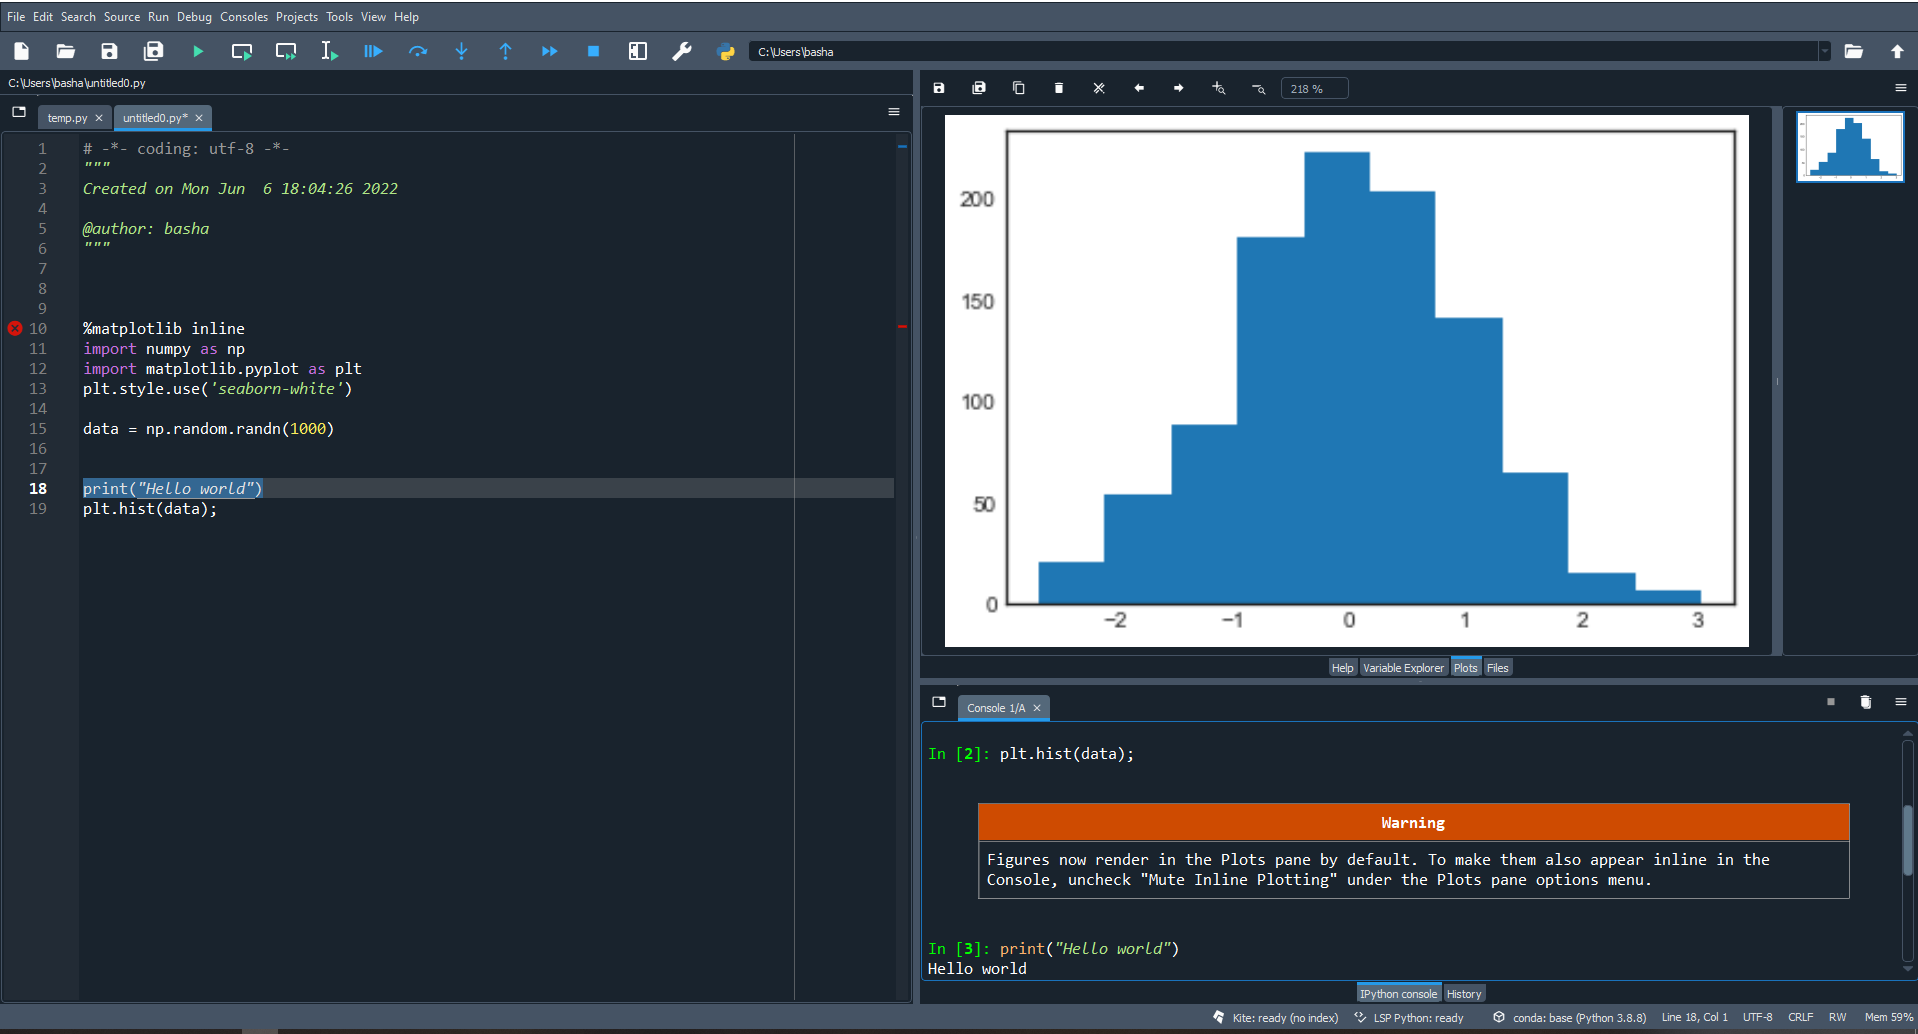
\includegraphics[width=1\linewidth]{Seminar_1_images/Spyder.PNG}
\end{figure}
\end{frame}

%-------------------------------------------------------------
\subsection{Verifying the folder structure }
%-------------------------------------------------------------
%-------------------------------------------------------------
\begin{frame}
\frametitle{Verifying the working folder structure}
\begin{figure}
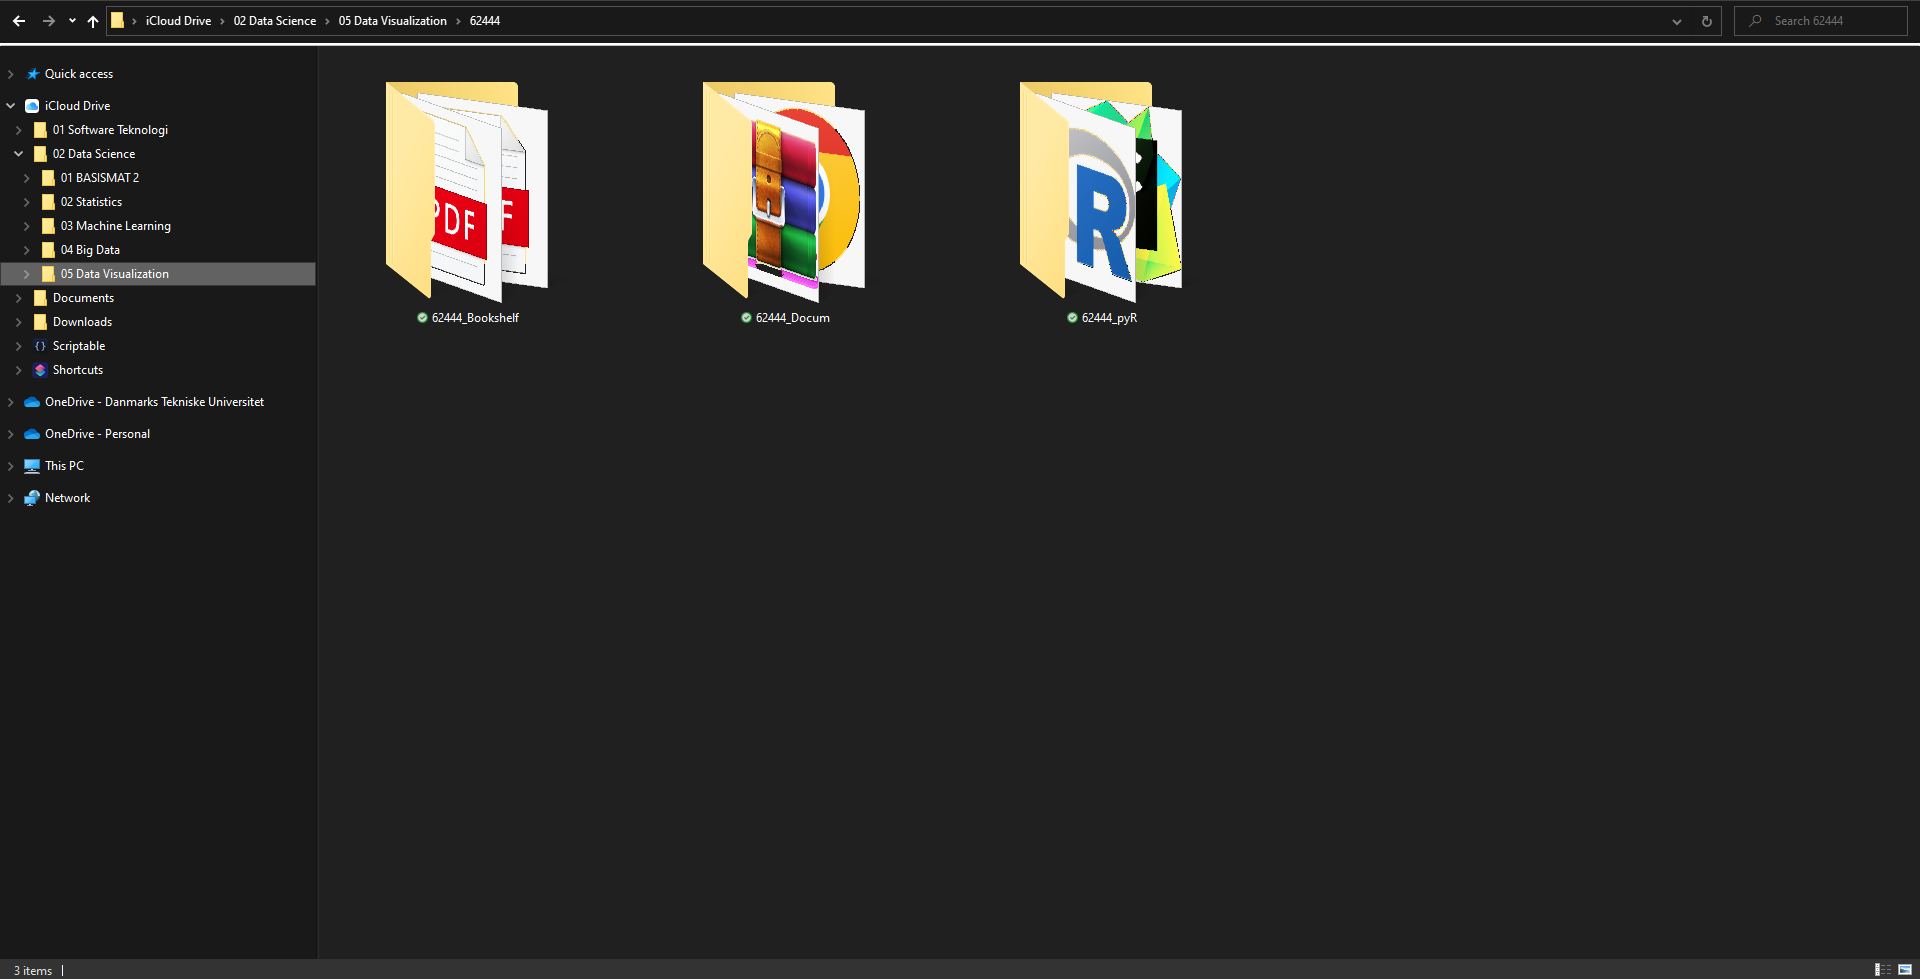
\includegraphics[width=1\linewidth]{Seminar_1_images/file structure.PNG}
\end{figure}
\end{frame}
%-------------------------------------------------------------
% ##========================================================##
% ##                                                        ##
% ##                        Seminar 2                       ##
% ##                                                        ##
% ##========================================================##
\section{Seminar 2: Data visualization and Analysis using
Python/R Libraries on Laptop and Cloud}
%-------------------------------------------------------------
\begin{frame}[fragile] % Need to use the fragile option when verbatim is used in the slide
\frametitle{Seminar 2 - Table of Contents}

\begin{enumerate}
\item R/RStudio
\begin{itemize}
\item R Language elements
\item Graph Visualization 
\item A Selection of Visualization in R
\item Text Analysis and Visualization in R
\item RStudio Cloud
\item Vattenfall dataset visualization and analysis (part 01)
\end{itemize}

\item Python/Spyder enviroment
\begin{itemize}
\item Python Language elements
\item Python Libraries
\end{itemize}

\item Google CoLab

\end{enumerate}

\end{frame}
%-------------------------------------------------------------
\subsection{Data Visualization using R/RStudio} 
%-------------------------------------------------------------
\begin{frame}[fragile] % Need to use the fragile option when verbatim is used in the slide
\frametitle{Seminar 2 - An example using for loop in R to count the number of even numbers in a vector.}
\begin{example}[1.1]
\begin{verbatim}

x <- c(2,5,3,9,8,11,6)
count <- 0
for (val in x) {
if(val %% 2 == 0)
count = count+1
}
print(count)
\end{verbatim}
\end{example}
\begin{example}[1.1 output:]
\begin{verbatim}
[1] 3
\end{verbatim}
\end{example}
\end{frame}
%-------------------------------------------------------------

%-------------------------------------------------------------
\begin{frame}[fragile]
\frametitle{Seminar 2 - Using if-else-statement in R}
\begin{example}[1.2]
\begin{verbatim}

x <- -5
if(x > 0){
print("Non-negative number")
} else {
print("Negative number")
}

# Output:
[1] "Negative number"
\end{verbatim}
\end{example}
\end{frame}
%-------------------------------------------------------------
\begin{frame}[fragile] 
\frametitle{Seminar 2 - Using while loop in R to calculate factorial of a number}
\begin{example}[1.3]
\begin{verbatim}
n <- 5

factorial <- 1
i <- 1

while (i <= n)
{
  factorial = factorial * i
  i = i + 1
}
print(factorial)
}

# Output: [1] 120
\end{verbatim}
\end{example}
\end{frame}

%-------------------------------------------------------------
\begin{frame}
\frametitle{Seminar 2 - Graph Visualization in R  }
\textbf{Example 2.1: Colors}\\
In most R functions, we can use named colors, hex, or rgb values, output of this lines of codes is showing the result:\newline

plot(x=1:10, y=rep(5,10), pch=19, cex=5, col="\#FFFF00")
points(x=1:10, y=rep(6, 10), pch=19, cex=5, col="pink")
points(x=1:10, y=rep(4, 10), pch=19, cex=5, col=rgb(.255, .0, .255))
\begin{figure}
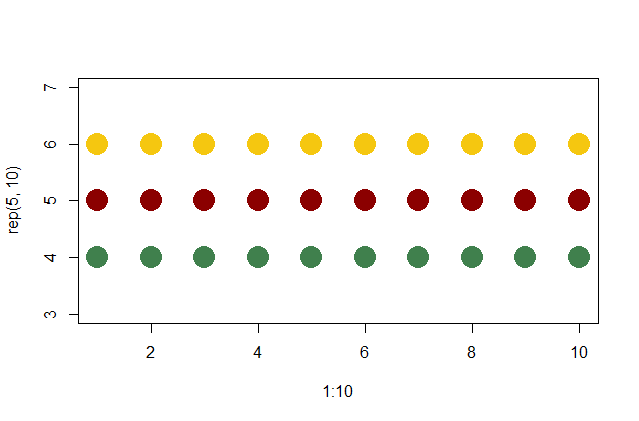
\includegraphics[width=0.5\linewidth]{Seminar_2_images/R/b Graph Visualization.png}
\end{figure}
\end{frame}
%-------------------------------------------------------------
\begin{frame}
\textbf{Example 2.2: Network layouts}\newline

Network layouts are algorithms that return coordinates for each node in a network.\newline
sample\_pa() function is used to generate a simple graph starting from one node and adding more nodes and links based on a preset level of preferential attachment (Barabasi-Albert model)
\begin{figure}
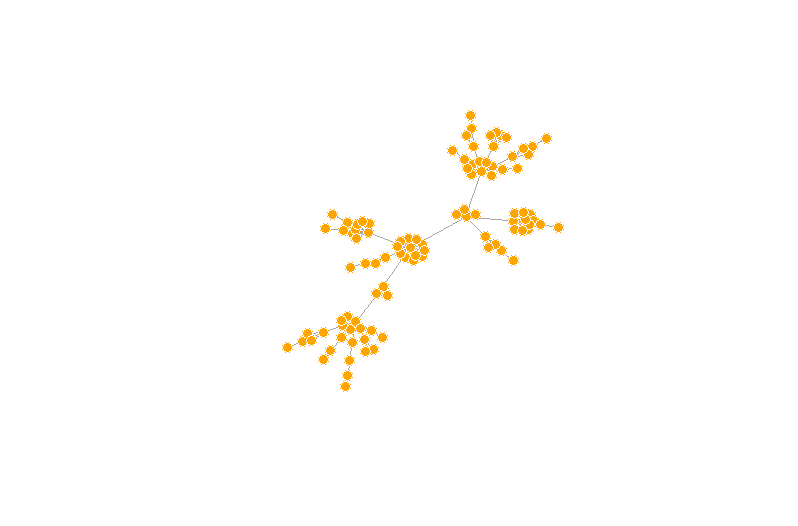
\includegraphics[width=0.8\linewidth]{Seminar_2_images/R/b network layout.png}
\end{figure}

\end{frame}

%-------------------------------------------------------------
\begin{frame}[fragile] 
\begin{example} [2.2: Network layouts code]
\begin{verbatim}
library(igraph)
net.bg <- sample_pa(100) 
V(net.bg)$size <- 8
V(net.bg)$frame.color <- "white"
V(net.bg)$color <- "orange"
V(net.bg)$label <- "" 
E(net.bg)$arrow.mode <- 0
plot(net.bg)
\end{verbatim}
\end{example}
\end{frame}

%-------------------------------------------------------------
\begin{frame}
\frametitle{Seminar 2 - A Selection of Visualizations in R}

\cite{Kabacoff2020} is used for preparing an R script which demonstrates the following types of visualizations:\newline
\begin{itemize}
\item Categorical Data
\begin{itemize}
\item Bar Charts
\item Pie Charts

\end{itemize}

\item Distributions
\begin{itemize}
\item Box Plots for Groups
\end{itemize}

\item Times Series

\item Scatter Plot
\end{itemize}
\end{frame}

%-------------------------------------------------------------
\begin{frame}
\frametitle{Seminar 2 - Categorical Data .... Bar plot}

\textbf{Example 3.1: Bar Chart}\\
The Marriage dataset contains the marriage records of 98 individuals in Mobile County, Alabama. Below, a bar chart is used to display the distribution of wedding participants by race.\newline 

\footnotesize
library(ggplot2)\\
data(Marriage, package = "mosaicData")\newline 
\# plot the distribution of race\\
ggplot(Marriage, aes(x = race)) + \\
\textcolor{white}{---} geom\_bar()\\
\begin{figure}
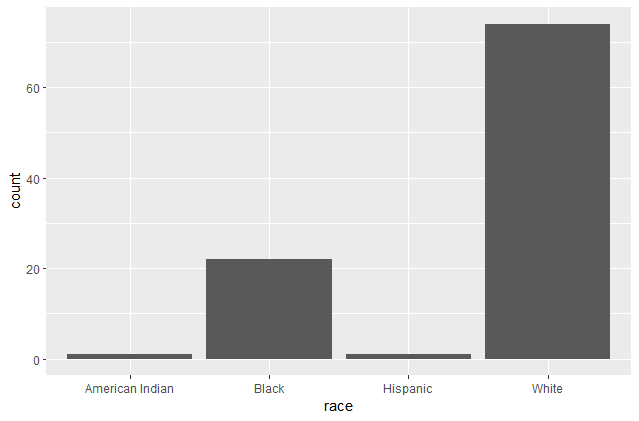
\includegraphics[width=0.4\linewidth]{Seminar_2_images/R/b Bar Charts.png}
\end{figure}
\end{frame}
%-------------------------------------------------------------
\begin{frame}
\frametitle{Seminar 2 - Categorical Data ... Pie Chart}
\begin{example} [3.2: Pie Chart]
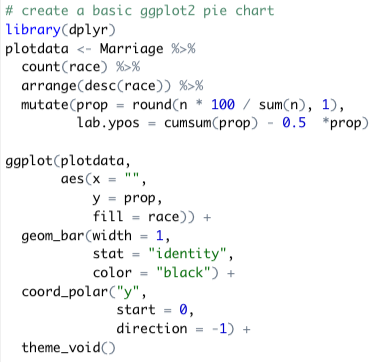
\includegraphics[width=0.4\linewidth]{Seminar_2_images/R/b pie_char_code.png}
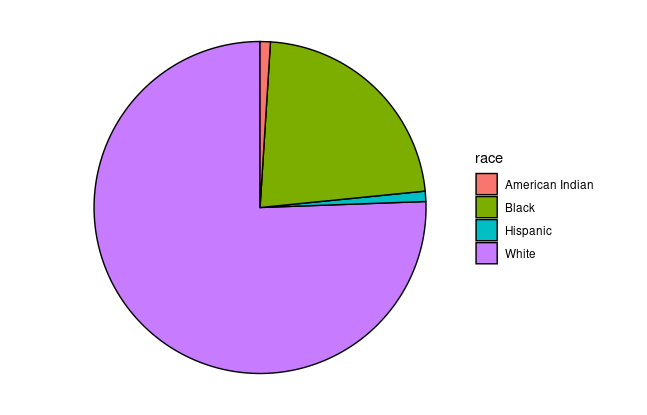
\includegraphics[width=0.59\linewidth]{Seminar_2_images/R/b pie-char.png}
\end{example}
\end{frame}
%-------------------------------------------------------------
\begin{frame}
\frametitle{Seminar 2 - Distribution ... Box plots }

\begin{example} [3.4: Box plots]
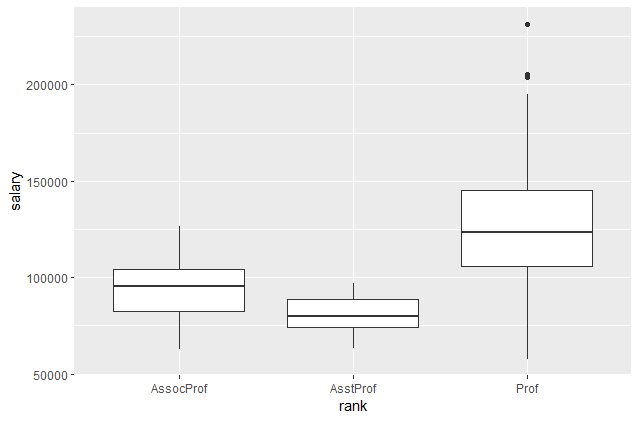
\includegraphics[width=0.8\linewidth]{Seminar_2_images/R/b boxplots.png}

\end{example}
\end{frame}

%-------------------------------------------------------------
\begin{frame}
\frametitle{Seminar 2 - Times Series }
A time series is a set of quantitative values obtained at successive time points. The intervals between time points (e.g., hours, days, weeks, months, or years) are usually equal.

Consider the Economics time series that come with the ggplot2 package. It contains US monthly economic data collected from January 1967 thru January 2015. Let’s plot personal savings rate (psavert). We can do this with a simple line plot.

\begin{example} [3.5: Time  Series]
library(ggplot2)\\
ggplot(economics, aes(x = date, y = psavert)) +\\
  geom\_line() +\\
  labs(title = "Personal Savings Rate",\\
       x = "Date",\\
       y = "Personal Savings Rate")

\end{example}
\end{frame}
%-------------------------------------------------------------
\begin{frame}
\frametitle{Output}
\begin{figure}
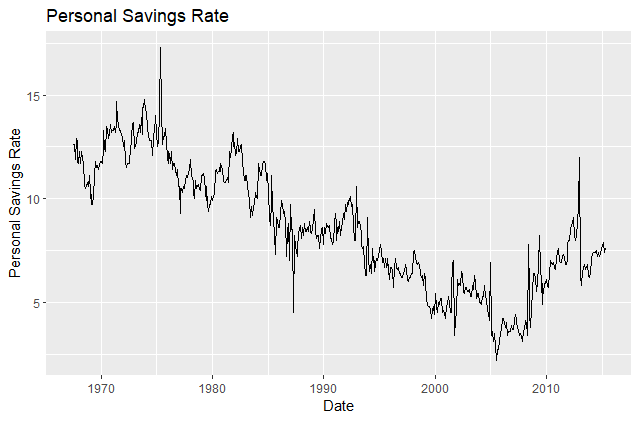
\includegraphics[width=1\linewidth]{Seminar_2_images/R/b time series.png}
\end{figure}
\end{frame}
%-------------------------------------------------------------
\begin{frame}
\frametitle{Seminar 2 - Quantitative vs Quantitative data ... Scatter Plot}

\begin{example} [3.5: scatter plot with line of best fit]

ggplot(data=Salaries, aes(x=yrs.since.phd, y=salary)) +\\ 
  geom\_point() + \newline
  geom\_smooth(method="lm", formula=y~x)
 
\end{example}
 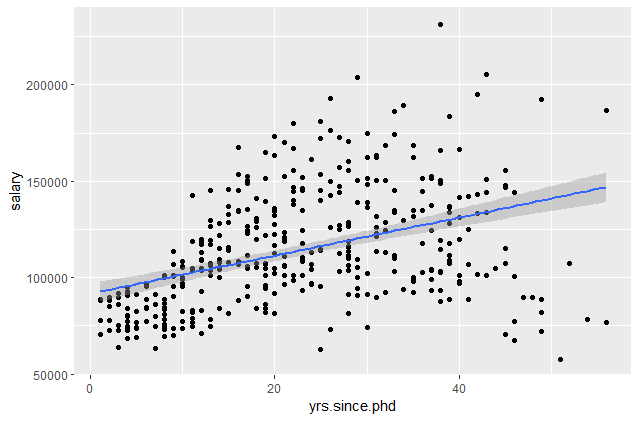
\includegraphics[width=0.6\linewidth]{Seminar_2_images/R/b scatterplot.png}
\end{frame}
%-------------------------------------------------------------
\begin{frame}
\frametitle{Seminar 2 - Text Analysis and Visualization in R ... Quanteda package}
\cite{Benoit2021} is used to verify the function of R-script for textual analysis.\newline

Quanteda is an R package for managing and analyzing textual data developed.\newline

Quanteda makes it easy to manage texts in the form of a corpus, defined as a collection of texts that includes document-level variables specific to each text, as well as meta-data.\newline


\end{frame}
%-------------------------------------------------------------
\begin{frame}
\frametitle{Quanteda R package}
\begin{figure}
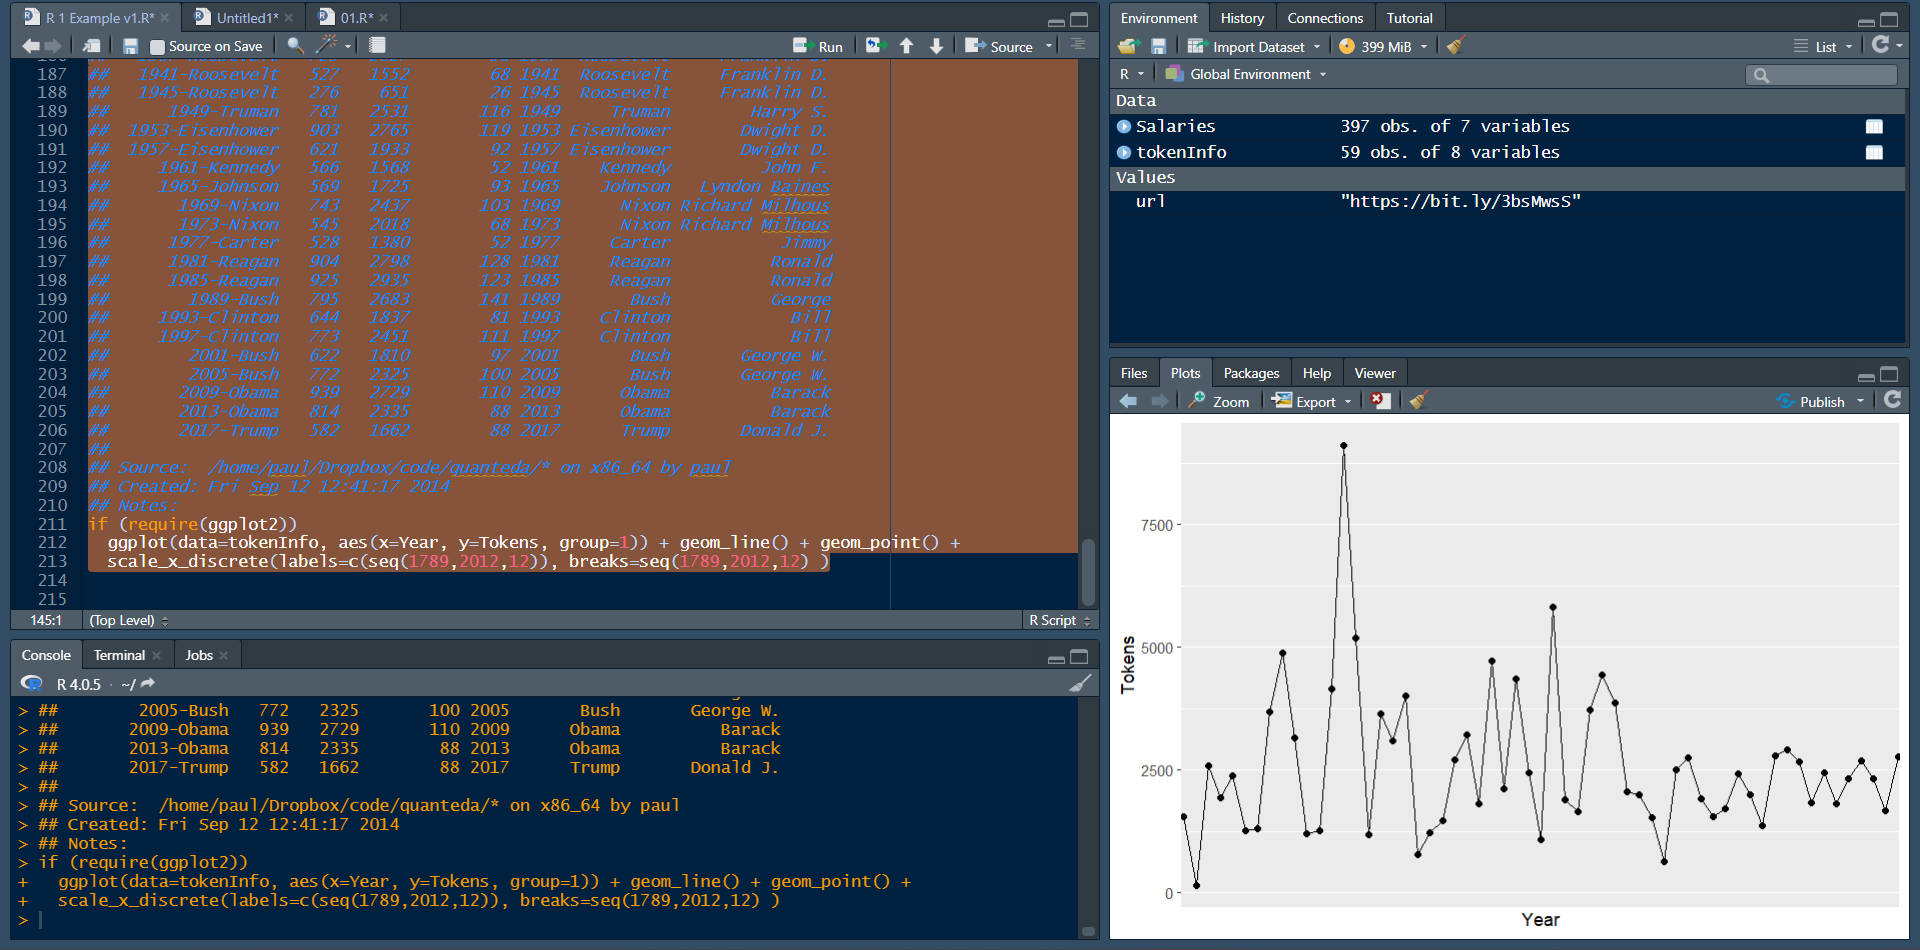
\includegraphics[width=1\linewidth]{Seminar_2_images/R/b quan.png}
\end{figure}
\end{frame}
%-------------------------------------------------------------
\begin{frame}
\frametitle{Seminar 2 - RStudio Cloud}
Example of how some of the R scripts developed can run on RStudio.Cloud.\newline

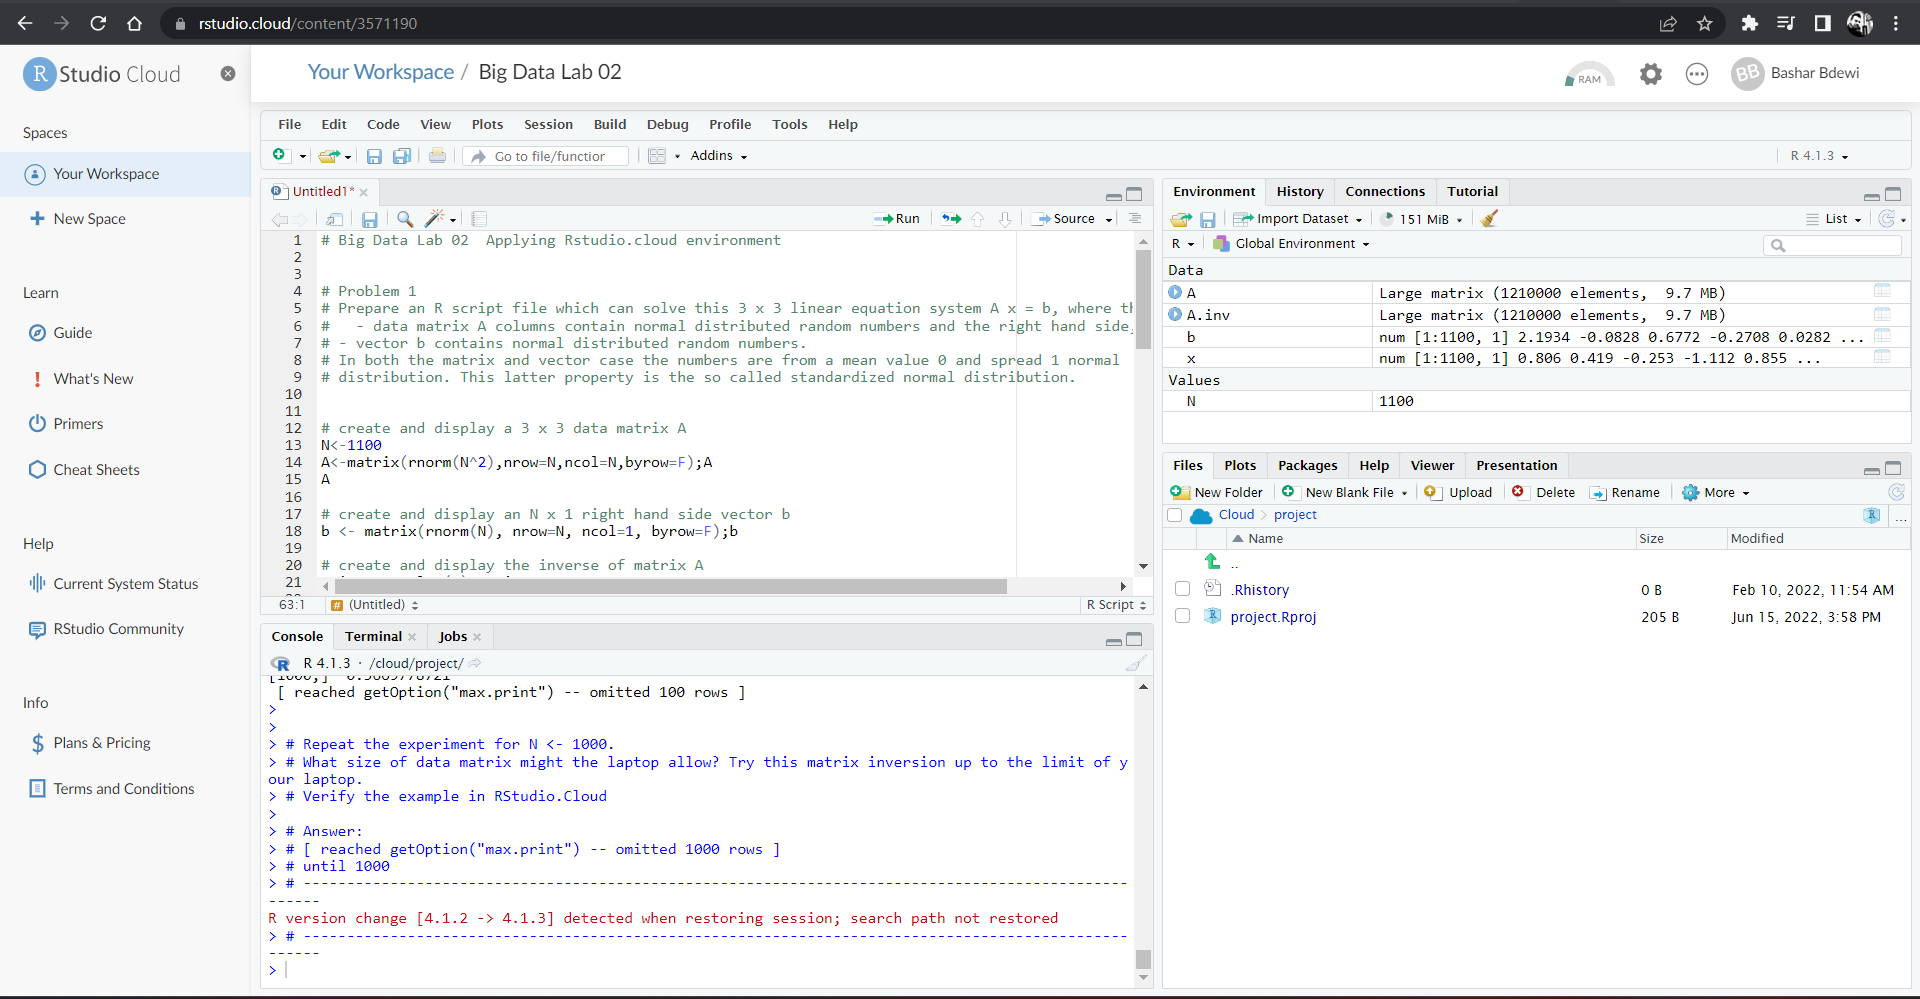
\includegraphics[width=1\linewidth]{Seminar_2_images/R/b Rcloud.png}


\end{frame}

%-------------------------------------------------------------
\subsection{Vattenfall dataset visualization and analysis using R} 
%-------------------------------------------------------------
\begin{frame}
\frametitle{Seminar 2 - Vattenfall dataset visualization and analysis using R}


We need to know what type of variables we are working with to choose the right statistical test for our data and interpret the results.\\\newline
.\\
In Vattenfall dataset all variables except "Turbine Stop Date" and "Component Exchange Date" are categorical data.
\end{frame}
%-------------------------------------------------------------
\begin{frame}[fragile] % Need to use the fragile option when verbatim is used in the slide
\frametitle{Vattenfall dataset Visualization\_Grouped bar plot}

\begin{example} [Grouped bar plot]
\# grouped bar plot\\

ggplot(data=wtf.df, aes(x=Component.Failed, fill=Park.Type)) + 
  geom\_bar(position="dodge")
\end{example}
\end{frame}
%-------------------------------------------------------------

\begin{frame}
\frametitle{Grouped bar plot\_"Component Failed" Vs. "Park Type"}


\begin{figure}
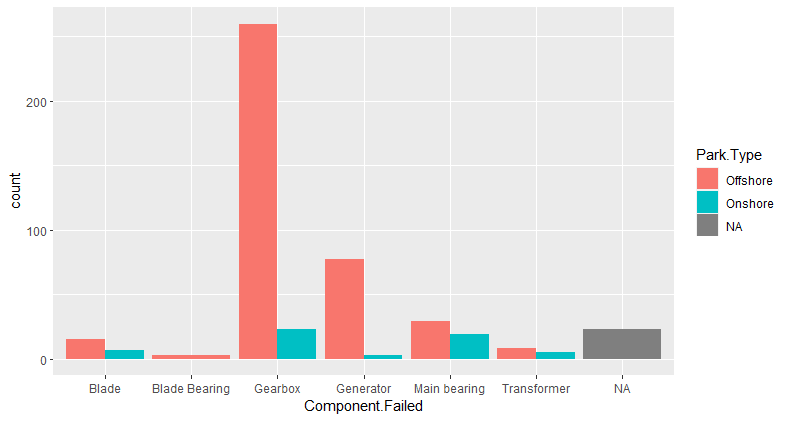
\includegraphics[width=1\linewidth]{Seminar_2_images/R/b vatten 1.png}
\end{figure}
\end{frame}
%-------------------------------------------------------------
\begin{frame}
\frametitle{Grouped bar plot\_"Component Failed" Vs. "Park Type"  (Graph Analysis)}
When plotting the relationship between two categorical variables, stacked,
grouped, or segmented bar charts are typically used.
Here is example of grouped bar charts, that place bars for the second
categorical variable side-by-side.\\ To create a grouped bar plot we use the
position = ”dodge” option.\\ 
We plotted plot the relationship between ”Component Failed” & ”Park Type”\newline

We can see here that the Gearbox is the most risky component and the offshore is the most difficult place.\\

\end{frame}
%-------------------------------------------------------------
\subsection{Data Visualization using Python\_Spyder} % Section
%-------------------------------------------------------------
\begin{frame}
\frametitle{Seminar 2 - Python Language elements}

\begin{itemize}
\item \textbf{for-loop}\newline
   \begin{figure}
   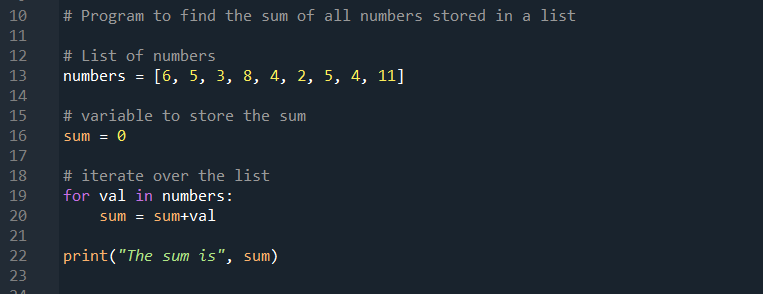
\includegraphics[width=0.9\linewidth]{Seminar_2_images/Python/for.png} 
   \end{figure}
\end{itemize}
 output: The sum is 48
\end{frame}   
%-------------------------------------------------------------
\begin{frame}[fragile]
\frametitle{Seminar 2 - Python Language elements }
\begin{itemize}
\item \textbf{if-statement}\newline
 \begin{figure} 
   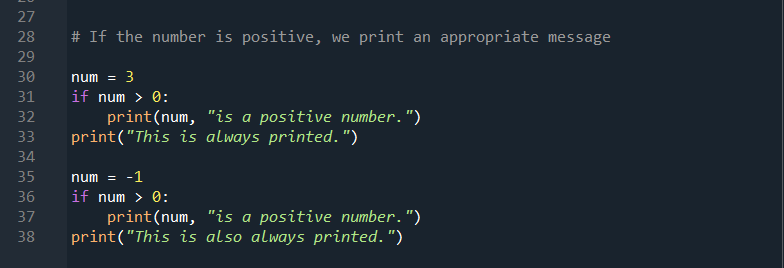
\includegraphics[width=0.9\linewidth]{Seminar_2_images/Python/b py 1.png} 
   \end{figure} 
   output :\newline 3 is a positive number.\newline
             This is always printed.\newline
             This is also always printed.\newline
\end{itemize}
\end{frame}

\begin{frame}[fragile]
\frametitle{Seminar 2 - Python Language elements }
\begin{itemize}
\item \textbf{while-loop}\newline

 \begin{figure} 
   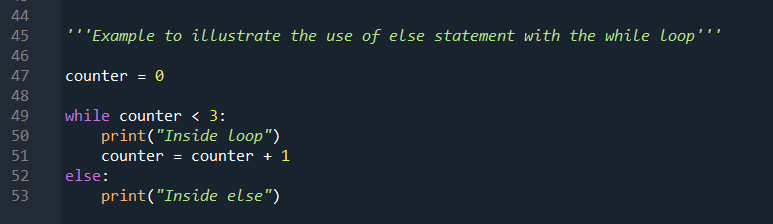
\includegraphics[width=0.8\linewidth]{Seminar_2_images/Python/b py 2.png}
   \end{figure}
   output:\newline Inside loop
Inside loop\newline
Inside loop\newline
Inside else\newline

\end{itemize}
\end{frame}

\begin{frame}[fragile]
\frametitle{Seminar 2 - Python Language elements }
\begin{itemize}

\item \textbf{Python function call}\newline
 \begin{figure} 
   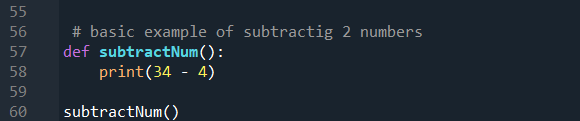
\includegraphics[width=0.8\linewidth]{Seminar_2_images/Python/b py 3.png}
   \end{figure}
   output: 30
\end{itemize}
\end{frame}
%-------------------------------------------------------------
\begin{frame}
\frametitle{Seminar 2 - Python Libraries}
\begin{itemize}
\item \textbf{matplotlib:}\newline
Collection of functions that make matplotlib work like MATLAB.
Each pyplot function makes a change to a figure: creates a figure, creates a plotting area in a figure, decorates the plot with labels, etc.
\begin{figure}
\centering

   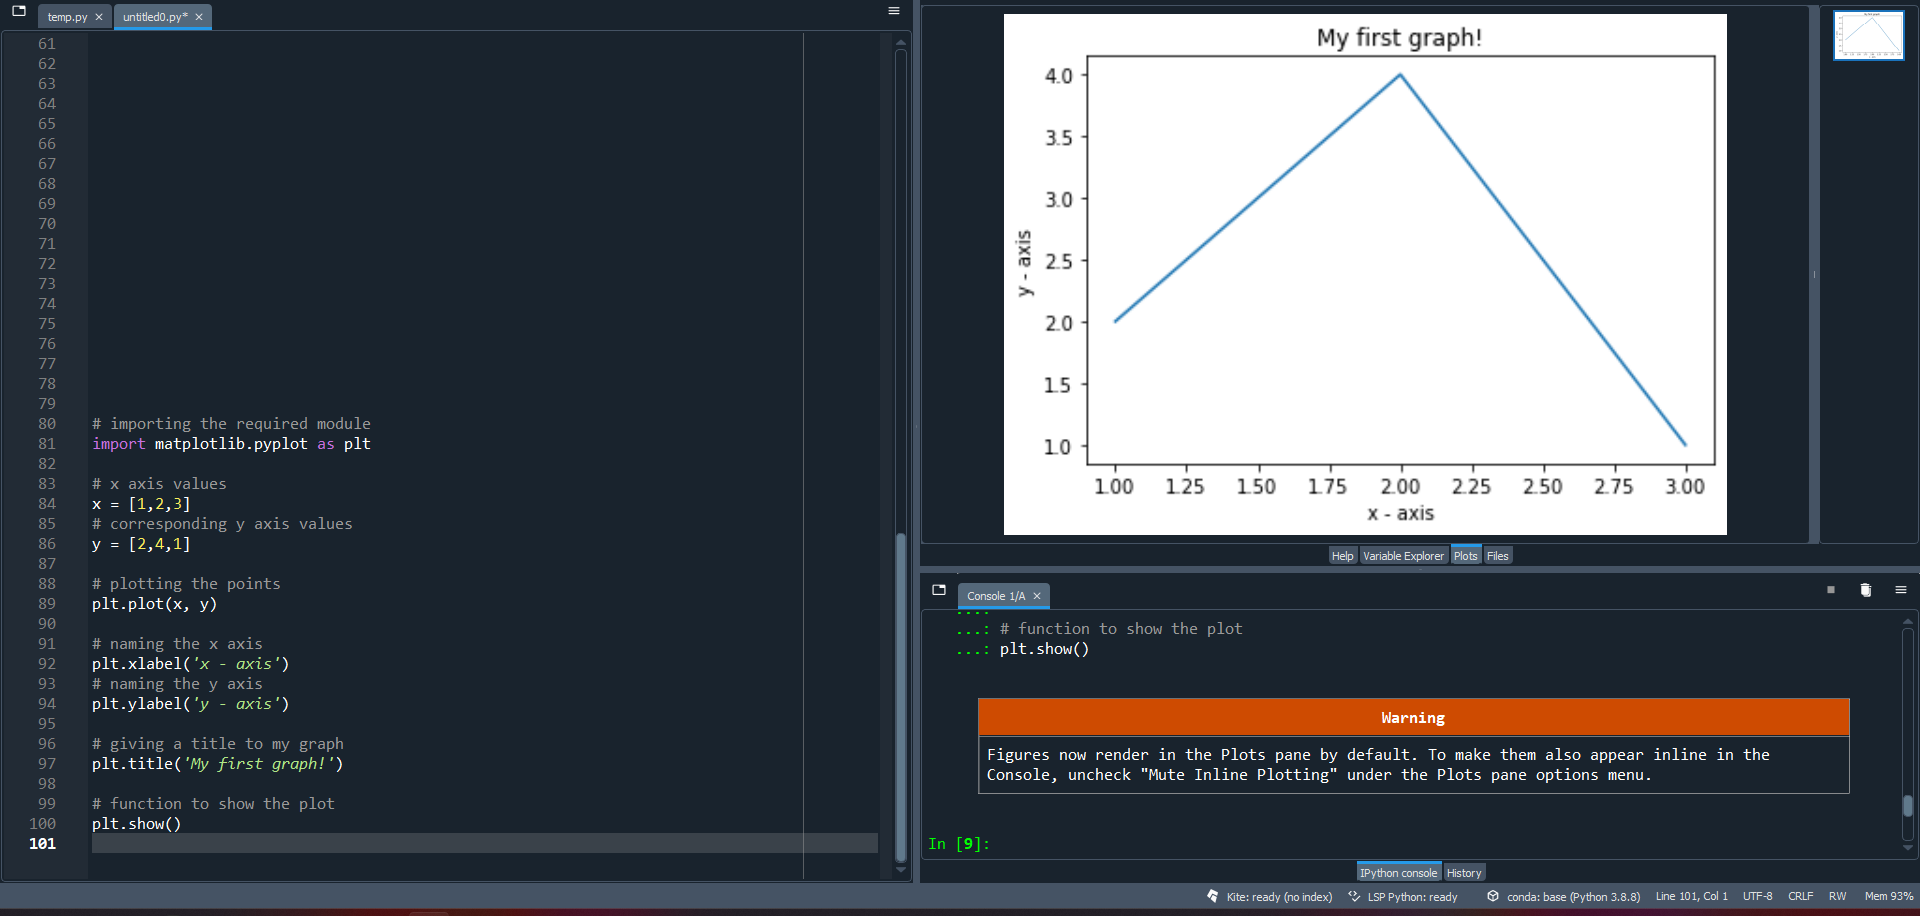
\includegraphics[width=0.9\linewidth]{Seminar_2_images/Python/b py 4.png}

\end{figure}
\end{itemize}
\end{frame}
%-------------------------------------------------------------
\begin{frame}
\frametitle{Seminar 2 - Python Libraries}
\begin{itemize}
    \item \textbf{Scikit-Learn:}\newline
    Machine learning library, uses NumPy for high-performance linear algebra and array operations.
    Main tool areas/algorithms:\newline
    \begin{itemize}
        \item \underline{Dimensionality Reduction:}
        Techniques for reducing the number of input variables in training data.
        In high dimensional data, useful to reduce the dimensionality by projecting the data to a lower dimensional subspace which captures the “essence” of the data. Unsupervised machine learning.
         \begin{figure}
         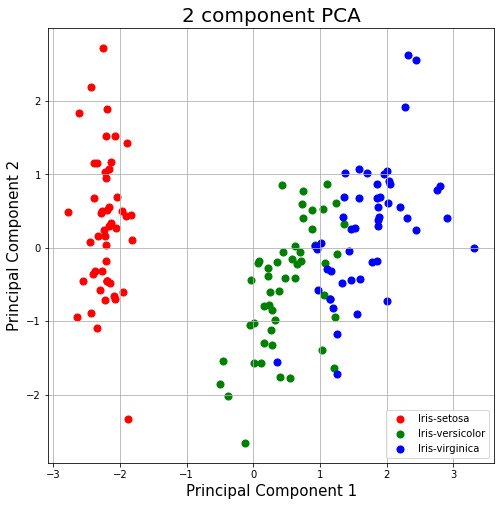
\includegraphics[width=0.4\linewidth]{Seminar_2_images/Python/b py 5.png}
         \label{Example mean-shift clustering algorithm}
         \end{figure}
   \end{itemize}
\end{itemize}
\end{frame}
%-------------------------------------------------------------
\begin{frame}[fragile]
\frametitle{Seminar 2 - Python Libraries}
    \begin{itemize}
        \item \underline{Clustering:}\newline
        Method of identifying and grouping similar data points in larger datasets.\newline
        Used to classify data into structures that are more easily understood and manipulated.
        Examples are unlabeled, unsupervised machine learning.
        Mean shift clustering: a centroid-based algorithm, which works by updating candidates for centroids to be the mean of the points within a given region.
         \begin{figure}
         \hspace{1.5cm}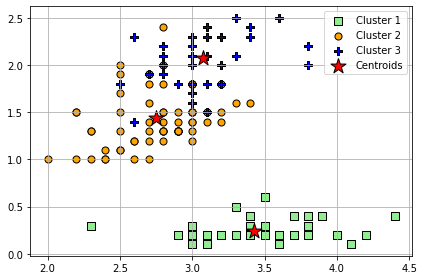
\includegraphics[width=0.5\linewidth]{Seminar_2_images/Python/b py 6.png}
       
         \end{figure}
    \end{itemize}
\end{frame}
%-------------------------------------------------------------
\begin{frame}[fragile]
\frametitle{Seminar 2 - Python Libraries}
    \begin{itemize}
        \item \underline{Regression:}\newline
        
        Statistical method for modelling relationship between a dependent variable with a given set of independent variables.
        \begin{figure}
        \hspace{1.5cm}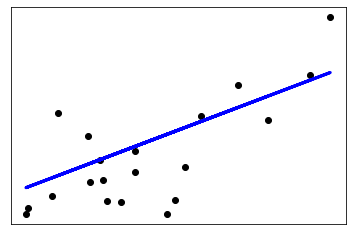
\includegraphics[width=0.5\linewidth]{Seminar_2_images/Python/b py 7.png}
       
        \end{figure}
    \end{itemize}
\end{frame}
%-------------------------------------------------------------

%-------------------------------------------------------------
\begin{frame}[fragile]
\frametitle{Seminar 2 - Python Libraries}
\begin{itemize}

    \item \textbf{Numpy:}\newline
    Numerical Python, for working with arrays.
    Facilitate advanced mathematical operations on large numbers of data.\newline
    Array objects that are 50x faster than traditional Python lists.
        \begin{figure}
        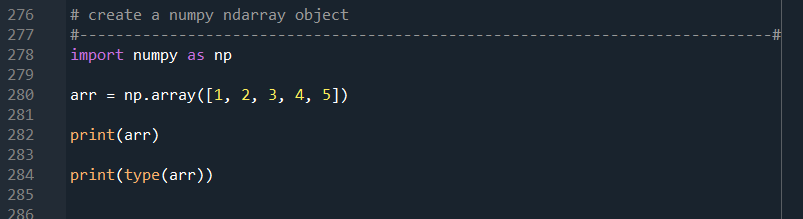
\includegraphics[width=0.65\linewidth]{Seminar_2_images/Python/numpy.png}
        \end{figure}

    \item \textbf{Plotly:}\newline
    For interactive, publication-quality graphs.Supports over 40 unique chart types covering a wide range of statistical, financial, geographic, scientific, and 3-dimensional use-cases.
        \begin{figure}
        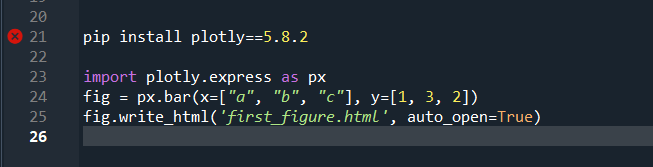
\includegraphics[width=0.65\linewidth]{Seminar_2_images/Python/b py 9.png}
        \end{figure}
\end{itemize}
\end{frame}

\begin{frame}[fragile]
\frametitle{Seminar 2 - Python Libraries}
\begin{itemize}
       \item \textbf{Pandas:}\newline
       Provides several different options for visualizing your data with .plot()\\
       Here it extracts the data from the .csv file into a Dataframe:
        \begin{figure}
        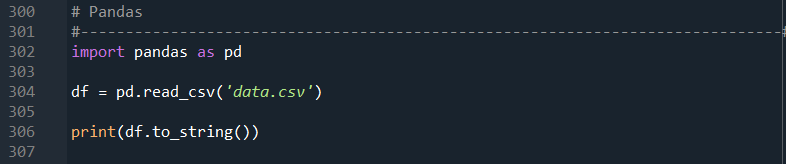
\includegraphics[width=1\linewidth]{Seminar_2_images/Python/pandas.png}
        \end{figure}
\end{itemize}
\end{frame}
%-------------------------------------------------------------
\subsection{Data Visualization using python\_Google CoLab} 
%-------------------------------------------------------------
\begin{frame}
\frametitle{Seminar 2 - Google CoLab}
visualization functions: 
\begin{itemize}
  \item line plots
        \begin{figure} 
        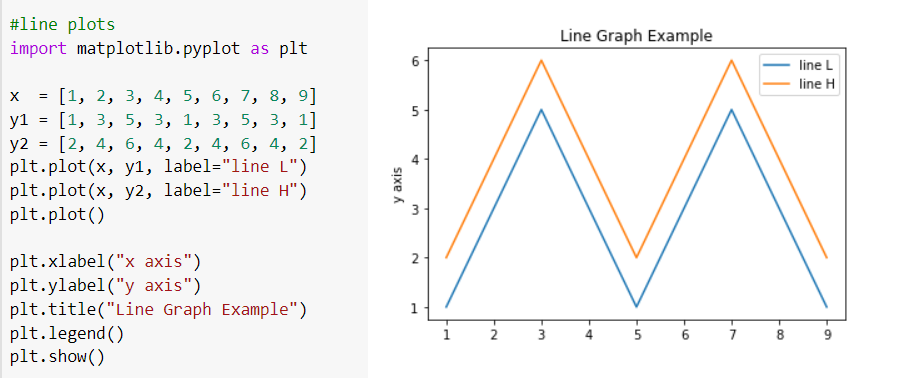
\includegraphics[width=0.7\linewidth]{Seminar_2_images/Google_Colab/lineplots.png}
        \end{figure}
  \item bar plots
        \begin{figure}
        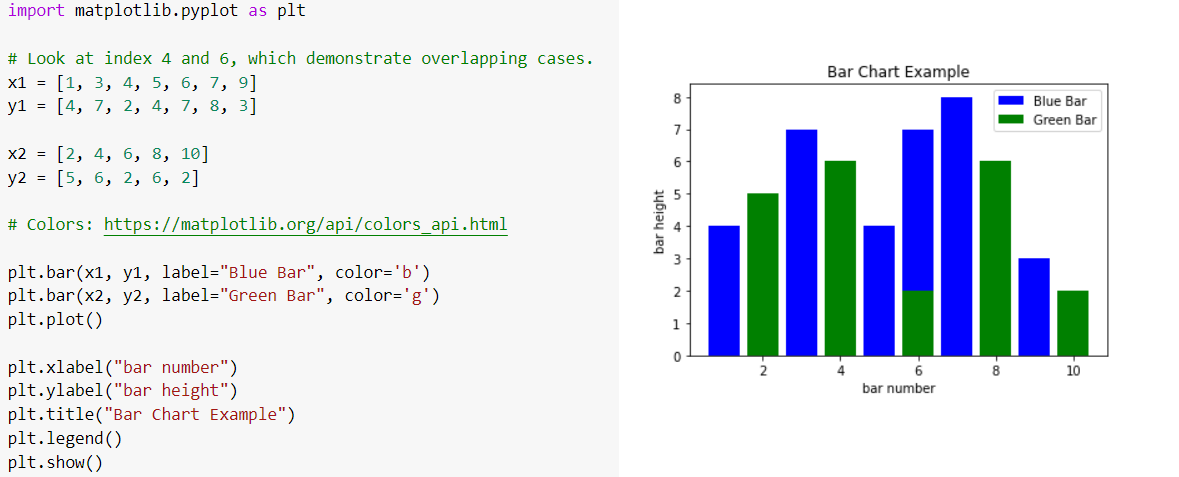
\includegraphics[width=0.7\linewidth]{Seminar_2_images/Google_Colab/barplots.png}
        \end{figure}
\end{itemize}
\end{frame}

\begin{frame}
\frametitle{Google CoLab}
visualization functions: 
\begin{itemize}
  \item histograms
        \begin{figure}
        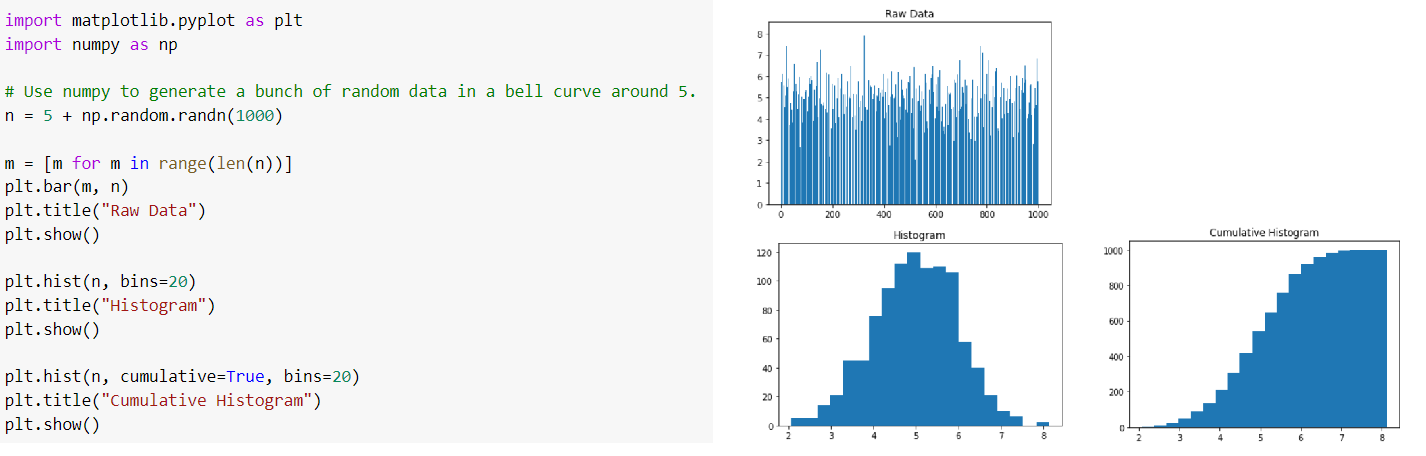
\includegraphics[width=0.7\linewidth]{Seminar_2_images/Google_Colab/histogram.png}
        \end{figure}
  \item pie chart
        \begin{figure}
        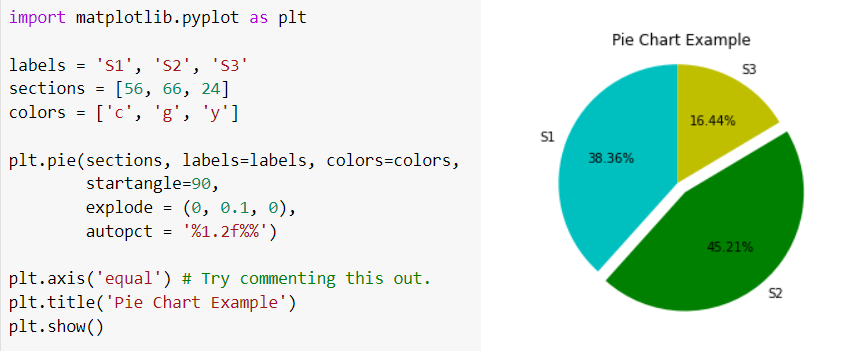
\includegraphics[width=0.7\linewidth]{Seminar_2_images/Google_Colab/pieChart.png}
        \end{figure}
\end{itemize}
\end{frame}

\begin{frame}
\frametitle{Google CoLab}
visualization functions: 
\begin{itemize}
  \item subplot
        \begin{figure}
        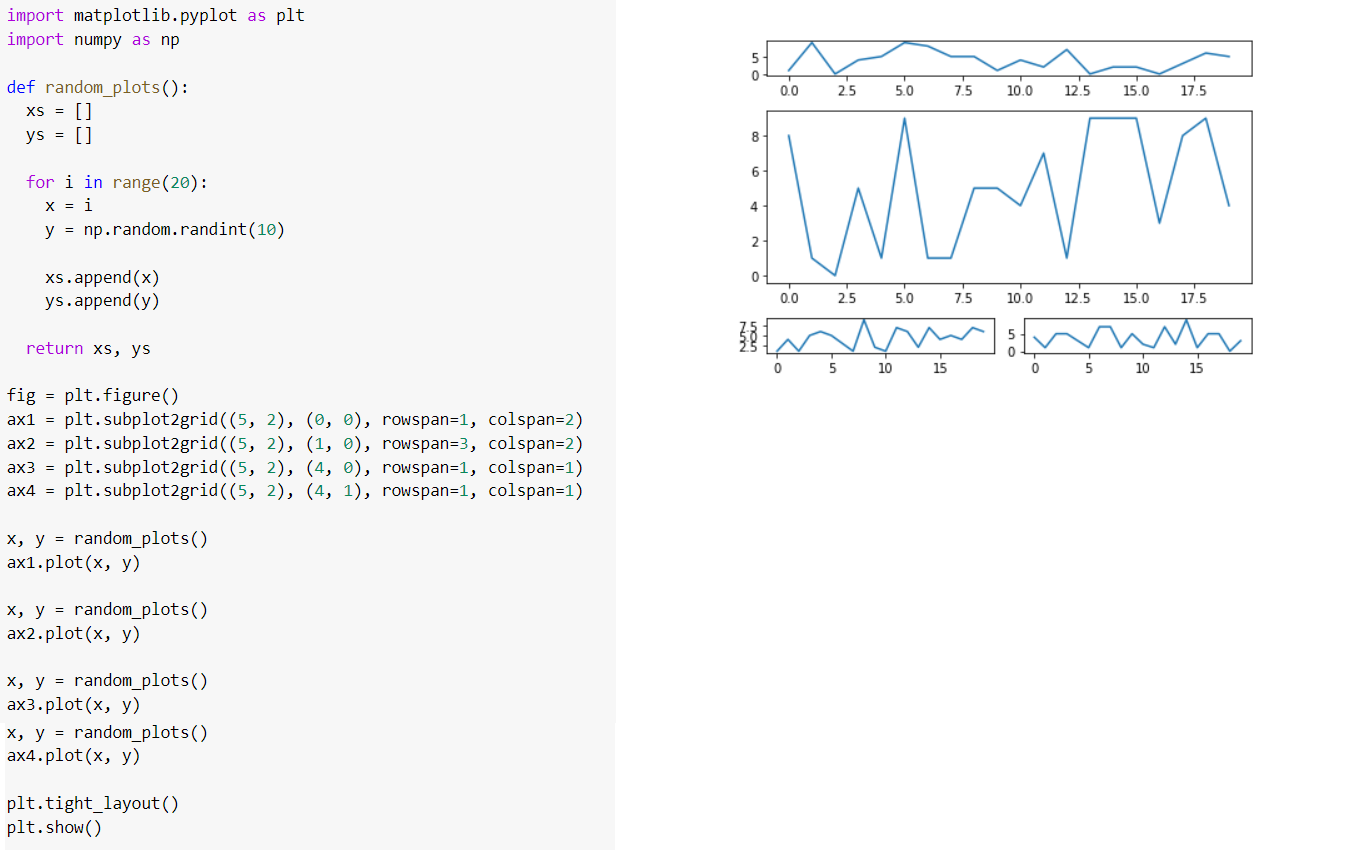
\includegraphics[width=0.8\linewidth]{Seminar_2_images/Google_Colab/subplotting.png}
        \end{figure}
\end{itemize}
\end{frame}

%-------------------------------------------------------------

%-------------------------------------------------------------




%-------------------------------------------------------------
% ##========================================================##
% ##                                                        ##
% ##                        Seminar 3                       ##
% ##                                                        ##
% ##========================================================##
\section{Seminar 3: Final Presentation}
%-------------------------------------------------------------

\begin{frame}[fragile] % Need to use the fragile option when verbatim is used in the slide
\frametitle{Seminar 3 - Table of Contents}


\begin{enumerate}
\footnotesize\item \textbf{R/RStudio}

\begin{itemize}
\item Bivariate Graphs in R
\item Vattenfall dataset visualization and analysis using R (part 02)
\item 3D visualization of data in R


\end{itemize}

\item \textbf{Python}
\begin{itemize}
\item Encoding categorical features in Python.
\item Bivariate Graphs in Python 
\item Vattenfall dataset visualization and analysis using Python
\end{itemize}

\item \textbf{Julia}\newline
A presentation of the language Julia

\end{enumerate}

\end{frame}
%-------------------------------------------------------------
\subsection{Data visualization in R/RStudio} 
%-------------------------------------------------------------

\begin{frame}[fragile] % Need to use the fragile option when verbatim is used in the slide
\frametitle{Categorical vs. Categorical}

\begin{example} [stacked bar chart]
ggplot(mpg, 
       aes(x = class, 
           fill = drv)) + 
  geom_bar(position = "stack)
\end{example}
\begin{figure}
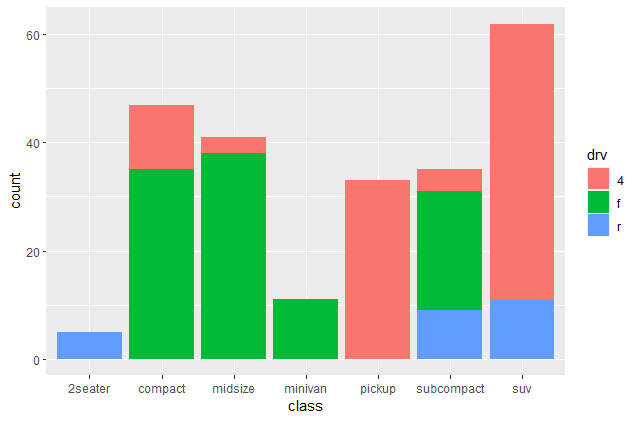
\includegraphics[width=0.8\linewidth]{Seminar_3_images/R/01.png}
\end{figure}
\end{frame}
%-------------------------------------------------------------
\begin{frame}[fragile] % Need to use the fragile option when verbatim is used in the slide
\frametitle{Categorical vs. Categorical}

\begin{example} [grouped bar plot]
Grouped bar charts place bars for the second categorical variable side-by-side. To create a grouped bar plot use the position = "dodge" option.
\end{example}
\begin{figure}

\includegraphics[width=0.7\linewidth]{Seminar_3_images/R/02.png}
\end{figure}
\end{frame}

%-------------------------------------------------------------

\begin{frame}[fragile] % Need to use the fragile option when verbatim is used in the slide
\frametitle{Categorical vs. Categorical}

\begin{example} [grouped bar plot preserving zero count bars]
Side-by-side bar chart with zero count bars retained
\end{example}
\begin{figure}
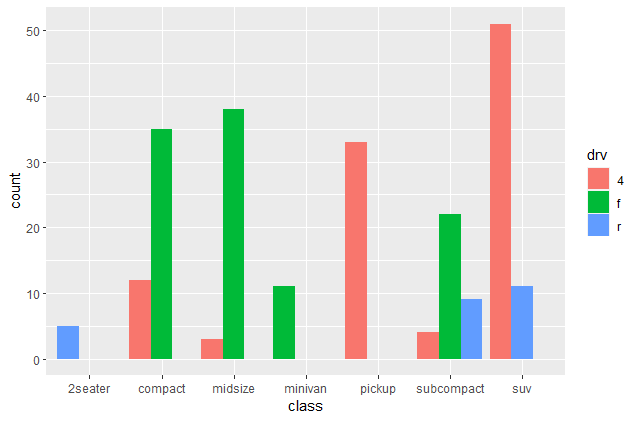
\includegraphics[width=0.8\linewidth]{Seminar_3_images/R/03.png}
\end{figure}
\end{frame}

%-------------------------------------------------------------

\begin{frame}[fragile] % Need to use the fragile option when verbatim is used in the slide
\frametitle{Categorical vs. Categorical}

\begin{example} [bar plot, with each bar representing 100%, 
reordered bars, and better labels and colors]
Segmented bar chart with improved labeling and color

\end{example}
\begin{figure}
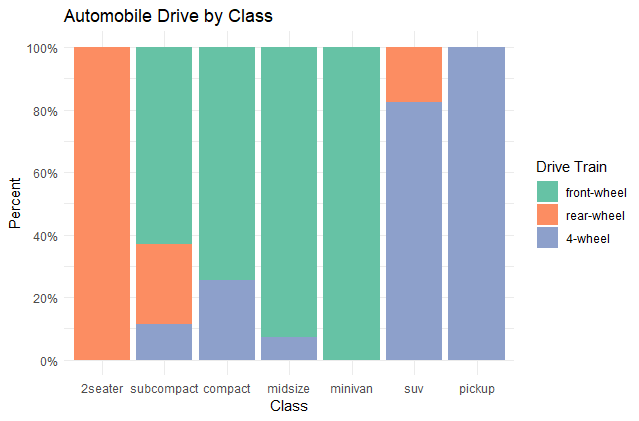
\includegraphics[width=0.75\linewidth]{Seminar_3_images/R/04.png}
\end{figure}
\end{frame}

%-------------------------------------------------------------

\begin{frame}[fragile] % Need to use the fragile option when verbatim is used in the slide
\frametitle{ Quantitative vs. Quantitative}

\begin{example} [enhanced scatter plot]

Scatterplot with color, transparency, and axis scaling

\end{example}
\begin{figure}
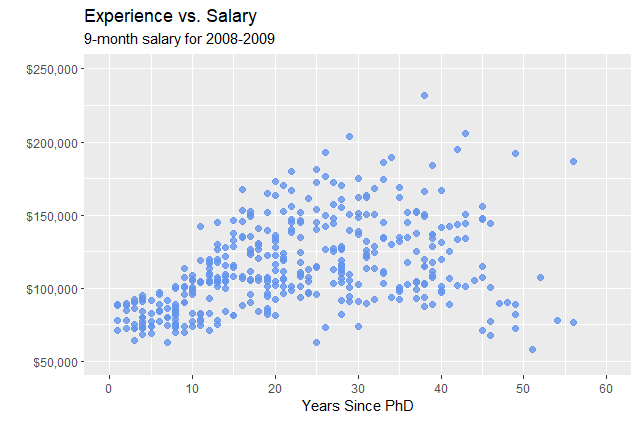
\includegraphics[width=0.8\linewidth]{Seminar_3_images/R/05.png}
\end{figure}
\end{frame}

%-------------------------------------------------------------

\begin{frame}[fragile] % Need to use the fragile option when verbatim is used in the slide
\frametitle{Quantitative vs. Quantitative}

\begin{example} [scatterplot with linear fit line]
It is often useful to summarize the relationship displayed in the scatterplot, using a best fit line.

\end{example}
\begin{figure}
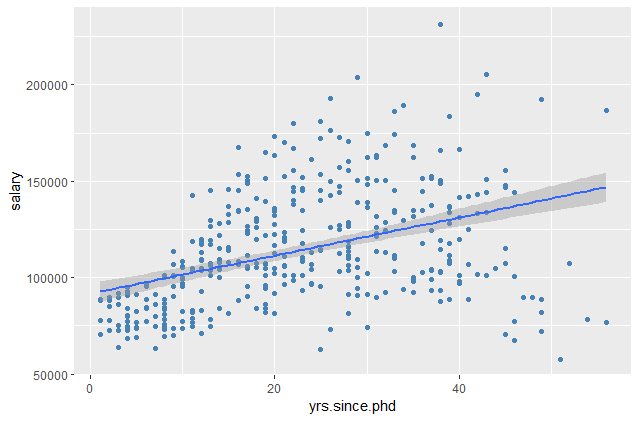
\includegraphics[width=0.75\linewidth]{Seminar_3_images/R/06.png}
\end{figure}
\end{frame}

%-------------------------------------------------------------

\begin{frame}[fragile] % Need to use the fragile option when verbatim is used in the slide
\frametitle{Quantitative vs. Quantitative}

\begin{example} [scatterplot with quadratic line of best fit]
Applying a quadratic fit to the salary dataset produces the following result

\end{example}
\begin{figure}
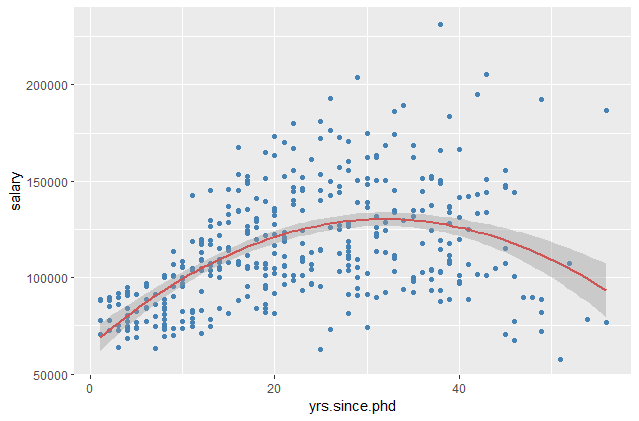
\includegraphics[width=0.8\linewidth]{Seminar_3_images/R/07.png}
\end{figure}
\end{frame}


%-------------------------------------------------------------

\begin{frame}[fragile] % Need to use the fragile option when verbatim is used in the slide
\frametitle{Categorical vs. Categorical}

\begin{example} [line plot with points]

When one of the two variables represents time, a line plot can be an effective method of displaying relationship.we’ll add points as well.

\end{example}
\begin{figure}
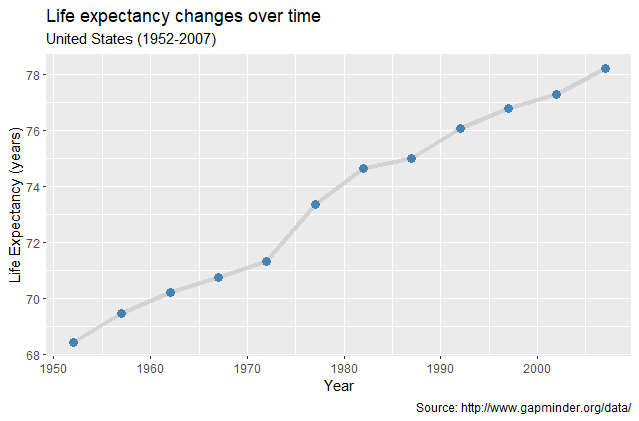
\includegraphics[width=0.8\linewidth]{Seminar_3_images/R/08.png}
\end{figure}
\end{frame}

%-------------------------------------------------------------

\begin{frame}[fragile] % Need to use the fragile option when verbatim is used in the slide
\frametitle{Categorical vs. Quantitative}

\begin{example} [plot mean salaries in a more attractive fashion]
We can make it more attractive with some options.
One limitation of such plots is that they do not display the distribution of the data - only the summary statistic for each group. Grouped kernel density plots correct this limitation to some extent.


\end{example}
\begin{figure}
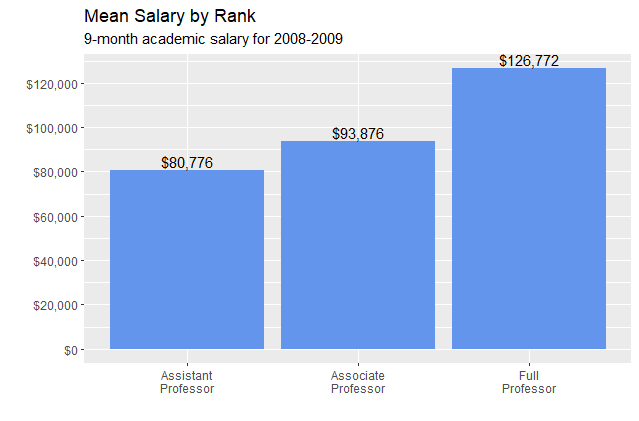
\includegraphics[width=0.6\linewidth]{Seminar_3_images/R/09.png}
\end{figure}
\end{frame}

%-------------------------------------------------------------

\begin{frame}[fragile] % Need to use the fragile option when verbatim is used in the slide
\frametitle{Categorical vs. Quantitative}

\begin{example} [plot the distribution of salaries 
 by rank using kernel density plots]
compare groups on a numeric variable by superimposing kernel density plots in a single graph.
 The graph makes clear that, in general, salary goes up with rank. However, the salary range for full professors is very wide
\end{example}
\begin{figure}
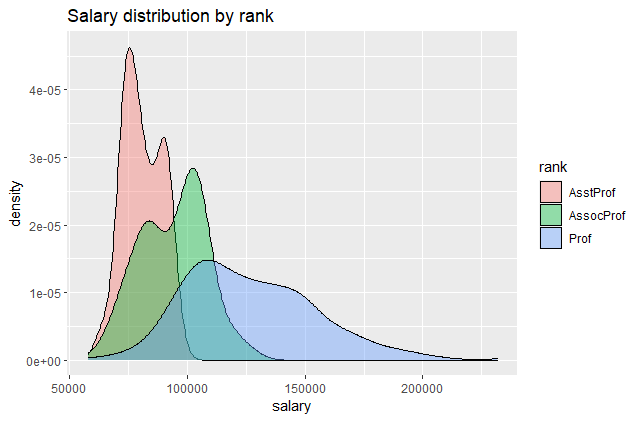
\includegraphics[width=0.6\linewidth]{Seminar_3_images/R/10.png}
\end{figure}
\end{frame}

%-------------------------------------------------------------

\begin{frame}[fragile] % Need to use the fragile option when verbatim is used in the slide
\frametitle{Categorical vs. Quantitative}

\begin{example} [plot the distribution of salaries by rank using boxplots]
Side-by-side box plots are very useful for comparing groups (i.e., the levels of a categorical variable) on a numerical variable.

\end{example}
\begin{figure}
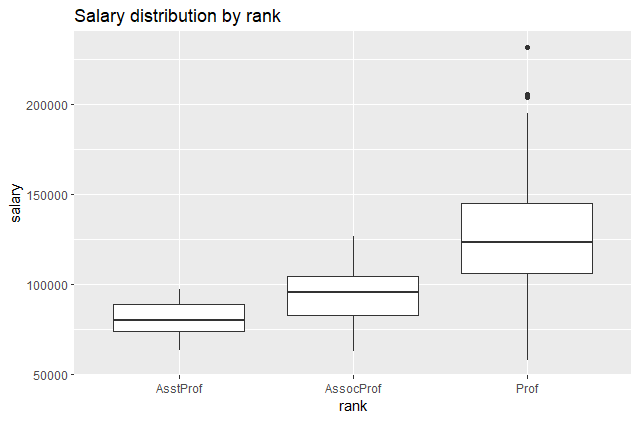
\includegraphics[width=0.75\linewidth]{Seminar_3_images/R/11.png}
\end{figure}
\end{frame}

%-------------------------------------------------------------

\begin{frame}[fragile] % Need to use the fragile option when verbatim is used in the slide
\frametitle{Categorical vs. Quantitative}

\begin{example} [plot the distribution of salaries 
 by rank using jittering]

It may be easier to visualize distributions if we add boxplots to the jitter plots.

\end{example}
\begin{figure}
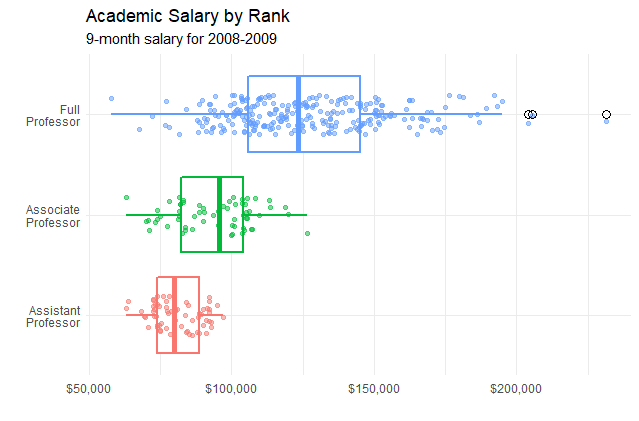
\includegraphics[width=0.75\linewidth]{Seminar_3_images/R/12.png}
\end{figure}
\end{frame}

%-------------------------------------------------------------

\begin{frame}[fragile] % Need to use the fragile option when verbatim is used in the slide
\frametitle{Interactive 3-D plots with RGL package}

\begin{example} [he plot3d function plots points within an RGL window]
The rgl package is used to produce interactive 3-D plots.The plot3d function plots points within an RGL window. It is similar to the classic plot function, but works in 3 dimensions.


\end{example}
\begin{figure}
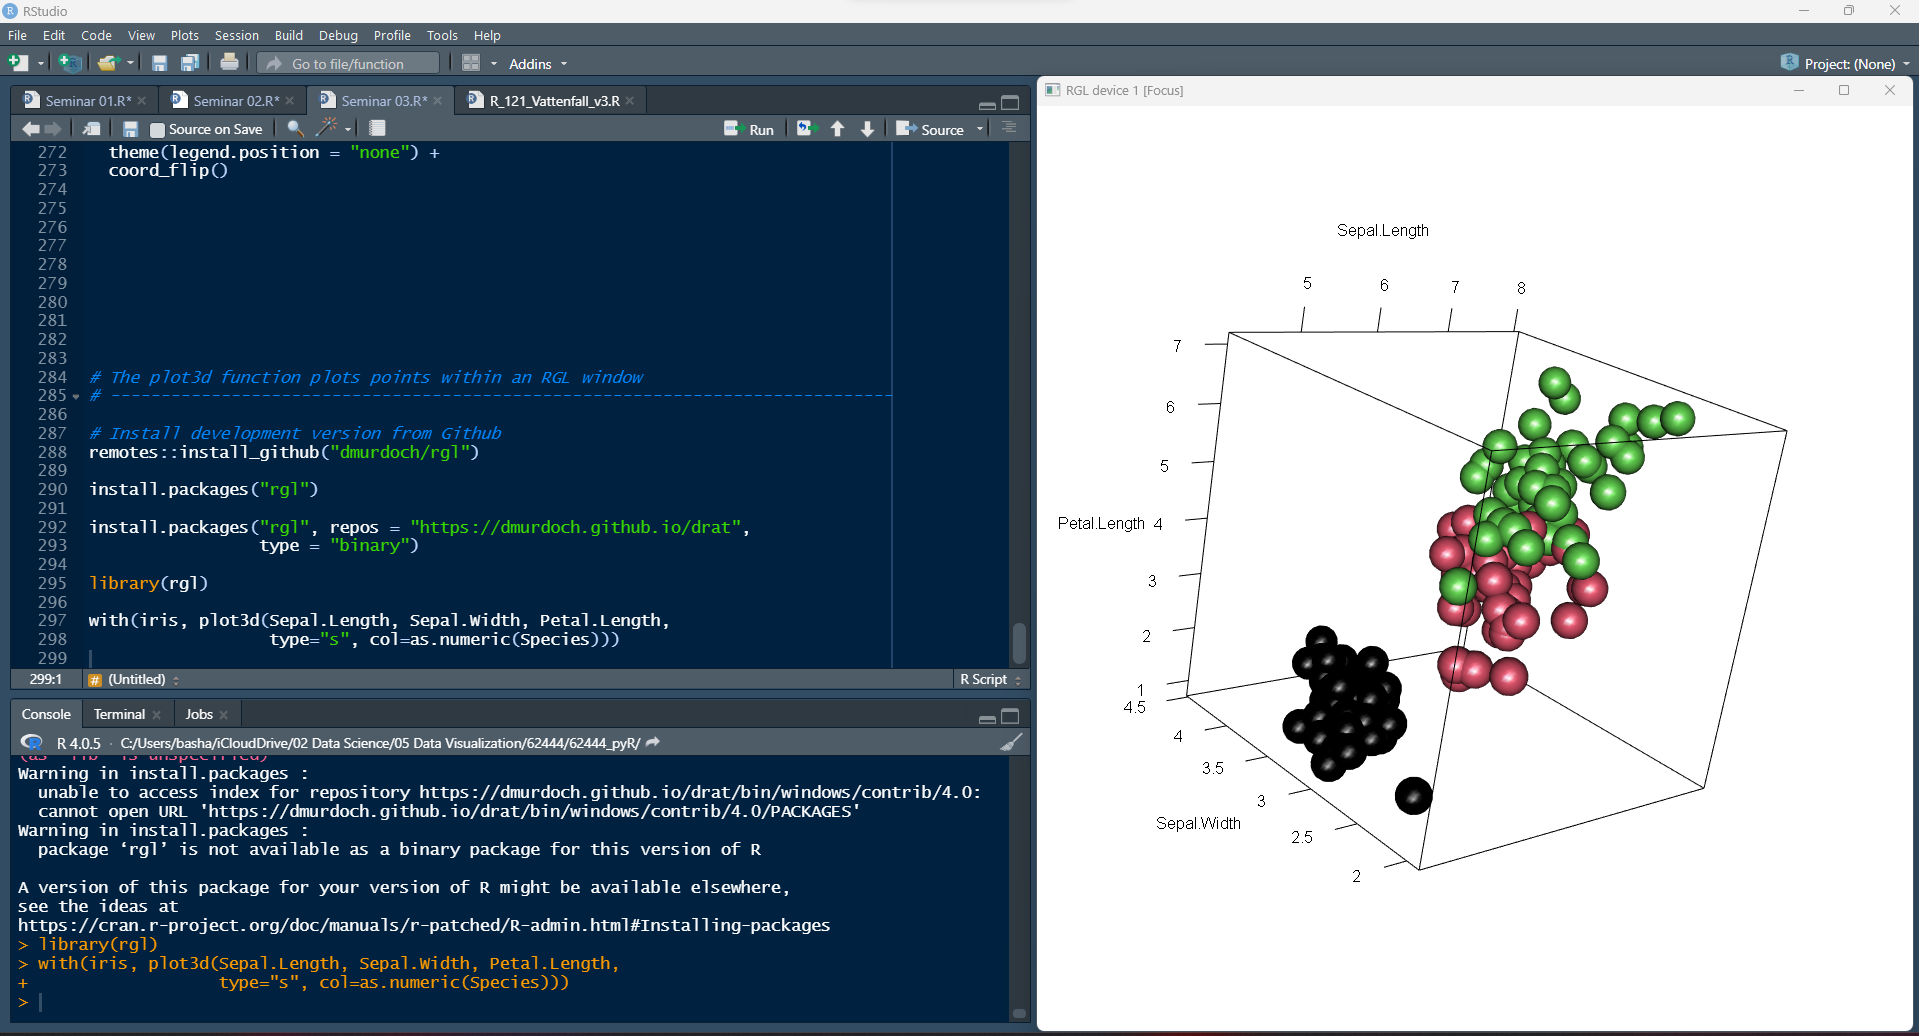
\includegraphics[width=0.8\linewidth]{Seminar_3_images/R/13.png}
\end{figure}
\end{frame}





\begin{frame}
\frametitle{Seminar 3 - The difference between categorical and quantitative data:}
\textbf{Quantitative} Quantitative data is defined as the value of data in the form of counts or numbers, that represents amounts like weight, height and age.\newline

\textbf{Categorical} variables is data which represents groups, like race, sex.\newline

We need to know what type of variables we are working with to choose the right statistical test for our data and interpret the results. e.g. in Vattenfall dataset all variables except "Turbine Stop Date" and "Component Exchange Date" are categorical data.
\end{frame}
%-------------------------------------------------------------



\begin{frame}
\frametitle{ "Component Failed" Vs. "Turbin platform"}
We can see here that the Gearbox is the most risky component and the offshore is the most difficult place. The following graph shows the distribution of Turbine Platform in different component failures, it shows that the most common failed is the V80-2MW.\\

\begin{figure}
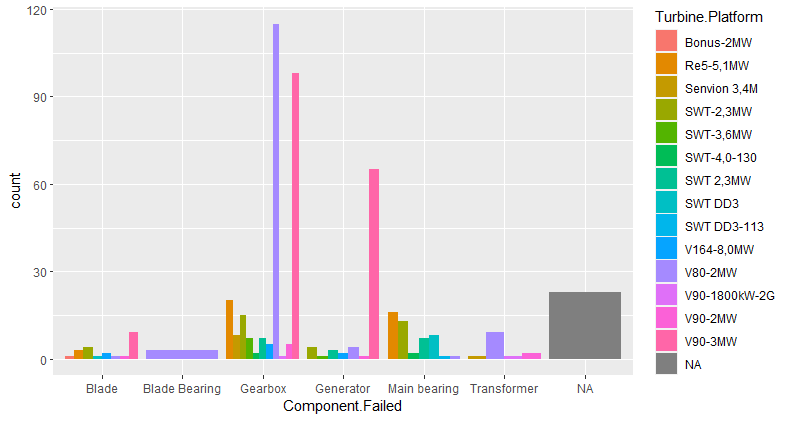
\includegraphics[width=0.8\linewidth]{Seminar_3_images/R/b vatten 2.png}
\end{figure}
\end{frame}


%-------------------------------------------------------------



\begin{frame}

\frametitle{"Turbine Stop Date" Vs. "Component Exchange Date"}

\begin{figure}
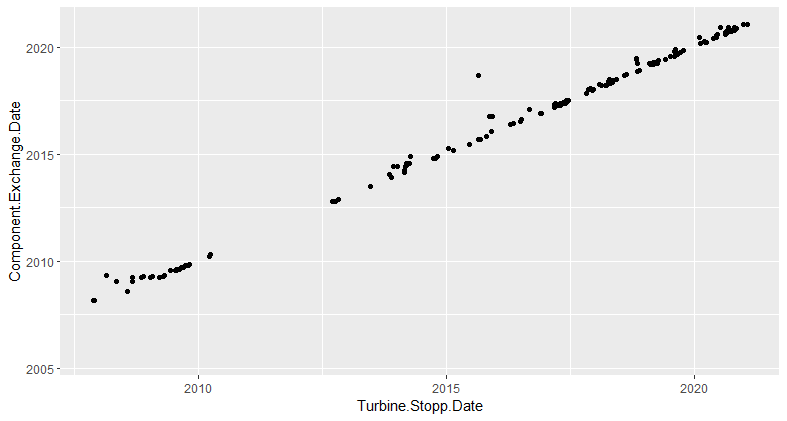
\includegraphics[width=0.9\linewidth]{Seminar_3_images/R/b vatten 3.png}
\end{figure}
\end{frame}

%-------------------------------------------------------------



%-------------------------------------------------------------
\begin{frame}[fragile] % Need to use the fragile option when verbatim is used in the slide
\frametitle{A descriptive analysis of the Vattenfall data set}
Descriptive statistics is the term given to the analysis of data that helps describe, show or summarize data in a meaningful way. By visualization of categorical and quantitative data on Vattenfall data set, we can conclude that there are more fails on the Gearbox component. The location will also effect the component failure, as the plot shows, the offshore is the most difficult place. The scatterplot shows that Component exchange will effect the life time of a turbine.

\end{frame}


%-------------------------------------------------------------
%-------------------------------------------------------------


%-------------------------------------------------------------
\subsection{Data visualization in Python} 
%-------------------------------------------------------------
\begin{frame}[fragile] % Need to use the fragile option when verbatim is used in the slide
\frametitle{Encoding categorical features}

\begin{example} [OrdinalEncoder]
Often features are not given as continuous values but categorical.To convert categorical features to such integer codes, we can use the OrdinalEncoder. This estimator transforms each categorical feature to one new feature of integers (0 to n_categories - 1)

\end{example}
\begin{figure}
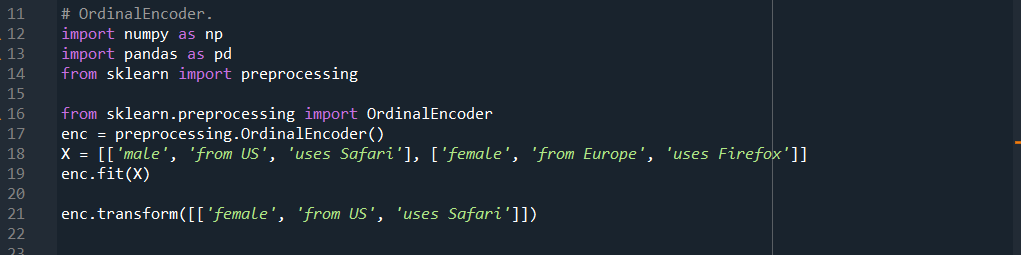
\includegraphics[width=0.8\linewidth]{Seminar_3_images/Python/01.png}
\end{figure}
Out: array([[0., 1., 1.]])
\end{frame}

%-------------------------------------------------------------

\begin{frame}[fragile] % Need to use the fragile option when verbatim is used in the slide
\frametitle{Encoding categorical features}

\begin{example} [OneHotEncoder]
to convert categorical features to features that can be used with scikit-learn estimators is to use a one-of-K or dummy encoding. This  encoding can be obtained with the OneHotEncoder.

\end{example}

\begin{figure}

\includegraphics[width=0.8\linewidth]{Seminar_3_images/Python/02.png}
\end{figure}
Out: 
array([[1., 0., 0., 1., 0., 1.],
       [0., 1., 1., 0., 0., 1.]])

\end{frame}
%-------------------------------------------------------------
\begin{frame}[fragile] % Need to use the fragile option when verbatim is used in the slide
\frametitle{seaborn: statistical data visualization}


\begin{example} [Categorical vs Categorical]
Bar plots

\end{example}

\begin{figure}
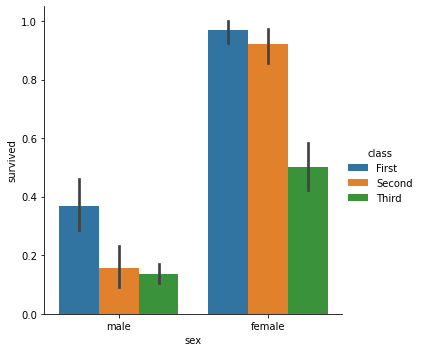
\includegraphics[width=0.6\linewidth]{Seminar_3_images/Python/03.png}
\end{figure}

\end{frame}

%-------------------------------------------------------------
\begin{frame}[fragile] % Need to use the fragile option when verbatim is used in the slide
\frametitle{seaborn: statistical data visualization}


\begin{example} [quantitative vs quantitative]
Plotting joint and marginal distributions. jointplot(), which augments a bivariate relatonal or distribution plot with the marginal distributions of the two variables. 

\end{example}

\begin{figure}
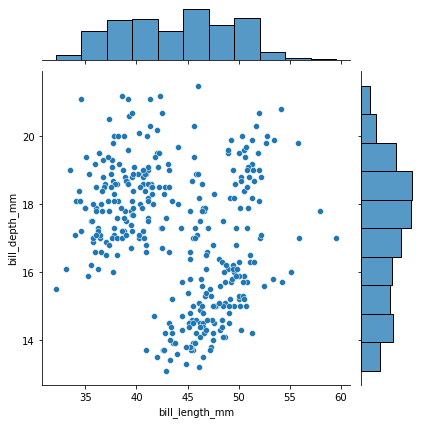
\includegraphics[width=0.4\linewidth]{Seminar_3_images/Python/04.png}
\end{figure}

\end{frame}

%-------------------------------------------------------------
\begin{frame}[fragile] % Need to use the fragile option when verbatim is used in the slide
\frametitle{seaborn: statistical data visualization}


\begin{example} [quantitative vs categorical]


\end{example}

\begin{figure}
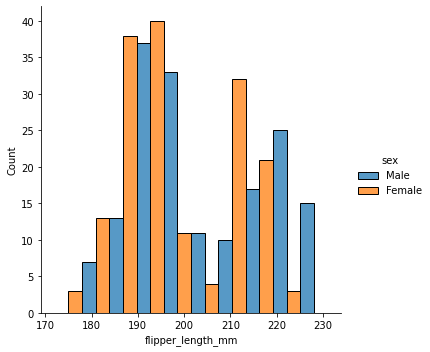
\includegraphics[width=0.6\linewidth]{Seminar_3_images/Python/05.png}
\end{figure}

\end{frame}

%-------------------------------------------------------------
\begin{frame}[fragile] % Need to use the fragile option when verbatim is used in the slide
\frametitle{Vattenfall dataset visualization and analysis}


\begin{example} ["Turbine Stopp Date" vs "Component Exchange Date"]


\end{example}

\begin{figure}
\includegraphics[width=0.6\linewidth]{Seminar_3_images/Python/06.png}
\end{figure}

\end{frame}
%-------------------------------------------------------------
\begin{frame}[fragile] % Need to use the fragile option when verbatim is used in the slide
\frametitle{Vattenfall dataset visualization and analysis}


\begin{example} ["Component Exchange Date "vs  hue="Component Failed"]


\end{example}

\begin{figure}
\includegraphics[width=0.6\linewidth]{Seminar_3_images/Python/07.png}
\end{figure}

\end{frame}














%-------------------------------------------------------------
\subsection{Data visualization in Julia} 
%-------------------------------------------------------------
\begin{frame}
\frametitle{Seminar 3 - Julia}
Why the language Julia?
\begin{itemize}
    \item Easy to use
     \item Free and open source
    \item Flexible dynamic language for high performance (fast)
    \item Brings high level dynamic and compiled languages together
   
   
\end{itemize}
Application areas:
\begin{itemize}
    \item Appropriate for scientific and numerical computing
    \item For building entire Applications and Microservices
\end{itemize}
Julia Language:
\begin{itemize}
    \item Has no classes / class-specific methods
    \item Standard Libraries and popular functions already included
\end{itemize}

\end{frame}
%-------------------------------------------------------------
% ##========================================================##
% ##                                                        ##
% ##                        References                      ##
% ##                                                        ##
% ##========================================================##
%%%%%%%%%%%%%%%%%%%%%%%%%%%%%%%%%%%%%%%%%%%%%%%%%%%%%%%%%%%%%%

\begin{frame}
\frametitle{References I}
\footnotesize{
\begin{thebibliography}{99} % Beamer does not support BibTeX so references must be inserted manually as below

\bibitem[Anaconda, 2022]{Anaconda2022} Anaconda Distribution (2022)
\newblock \emph{\href{https://www.anaconda.com}{www.anaconda.com}}
\newblock \emph{\href{https://www.anaconda.com/distribution/}{www.anaconda.com/distribution}}

\bibitem[Benoit, 2022]{Benoit2021} Kenneth Benoit (2022)
\newblock "Quantitative Analysis of Textual Data".
\newblock \emph{R-Package at CRAN 2022}
\newblock \emph{\url{https://cran.r-project.org/web/packages/quanteda/quanteda.pdf}}

\bibitem[Benoit, 2022a]{Benoit2022a} Kenneth Benoit (2022)
\newblock "vignettes quanteda: Quick Start Guide".
\emph{R-Package at CRAN 2022}
\newblock \emph{\url{https://cran.r-project.org/web/packages/quanteda/vignettes/quickstart.html}}

\bibitem[GoogleCoLab, 2022]{GoogleCoLab2022} Google CoLab (2022)
\newblock \emph{\url{https://colab.research.google.com}}

\end{thebibliography}
}
\end{frame}


\begin{frame}
\frametitle{References II}
\footnotesize{
\begin{thebibliography}{99} 



\bibitem[Horvath, 2020]{Horvath2020} Reka Horvath (2020)
\newblock "Plot With Pandas: Python Data Visualization for Beginners"
\newblock \emph{\url{https://realpython.com/pandas-plot-python/}}

\bibitem[Julia, 2022]{JuliaLang2022} The Julia Language (2022)
\newblock{\url{https://julialang.org/}}

\bibitem[Jupyter, 2021]{Jupyter2021} Jupyter Notebook (2021)
\newblock "The Jupyter Notebook".
\emph{\url{http://jupyter.org/}}

\bibitem[Kabacoff, 2020] {Kabacoff2020} Robert Kabacoff (2020)
\newblock  "Data Visualization with R".
\emph{\url{https://rkabacoff.github.io/datavis/}}

\bibitem[Machlis, 2019]{Machlis2019} Sharon Machlis (2019)
\newblock "Great R packages for data import, wrangling and visualization".
\newblock \emph{Computerworld, 2019}

\end{thebibliography}
}
\end{frame}
%%%%%%%%%%






\begin{frame}
\frametitle{References III}
\footnotesize{
\begin{thebibliography}{99} 


\bibitem[McKinney, 2022]{McKinney2022} Wes McKinney (2022)
\newblock "pandas: powerful Python data analysis toolkit"
\newblock \emph{\url{https://pandas.pydata.org/docs/pandas.pdf }}

\bibitem[M\"{u}ller, 2020]{Muller2020} Stephan M\"{u}ller, Kenneth Banoit (2020)
\newblock "quanteda - Cheat Sheet".
\newblock \emph{\url{https://www.rstudio.com/resources/cheatsheets/}}

\bibitem[Oetiker, 2021]{Oetiker2021} Tobias Oetiker, Hubert Partl, Irene Hyna and Elisabeth Schlegl (2021)
\newblock "The Not So Short Introduction to \LaTeX2e ".
\newblock \emph{\url{https://tobi.oetiker.ch/lshort/lshort.pdf}}

\bibitem[Ognyanova 2021]{Ognyanova2021} Katherine Ognyanova (2021)
\newblock "Network visualization with R".
\newblock \emph{\url{https://kateto.net/network-visualization}}
\end{thebibliography}
}
\end{frame}








\begin{frame}
\frametitle{References IV}
\footnotesize{
\begin{thebibliography}{99} 
\bibitem[Python, 2022]{PyPi2022} The Python Package Index (2022)
\newblock "The Python Package Index".
\newblock \emph{https://pypi.org/}

\bibitem[R, 2022]{R2022} The R Project for Statistical Computing (2022)
\newblock \emph{https://www.r-project.org/}

\bibitem[Ragan-Kelley, 2018]{Ragan-Kelley2018} Min Ragan-Kelley, Carol Willing, Jason Grout (2018)
\newblock "Jupyter: Tools for the Life Cycle of a Computational Idea".
\newblock \emph{SIAM News Volume 51, Issue 2 March 2018}

\bibitem[Rosling, 2018]{Rosling2018} Hans Rosling (2018)
\newblock "Gabminder".
\newblock \emph{\url{http://www.gapminder.org}}

\bibitem[RStudioCheatSheets, 2022]{RStudioCheatSheets2022} RStudio Cheat Sheets (2022)
\newblock \emph{\url{https://www.rstudio.com/resources/cheatsheets/}}

\end{thebibliography}
}
\end{frame}





\begin{frame}
\frametitle{References IIV}
\footnotesize{
\begin{thebibliography}{99} 
\bibitem[scikit-learn, 2022]{scikitLearn2022a} Machine Learning Map index (2022)
\newblock \emph{\url{https://scikit-learn.org/stable/tutorial/machine_learning_map/index.html}}

\bibitem[seaborn, 2022]{seaborn2022} The seaborn library for graphics in Python (2022).
\newblock \emph{\url{https://seaborn.pydata.org/}}

\bibitem[Stuart, 2022]{Stuart2022} Louis Stewart, Joseph Wright (2022)
\newblock "beamer – A LaTeX class for producing presentations and slides".
\newblock \emph{\url{https://github.com/josephwright/beamer}}

\bibitem[Tantau, 2022]{Tantau2022} Till Tantau, Joseph Wright, Vedran Mileti\'{c} (2022)
\newblock "The beamer class".
\newblock \emph{\url{http://tug.ctan.org/macros/latex/contrib/beamer/doc/beameruserguide.pdf}}


\bibitem[Torfs, 2014]{Torfs2014} Paul Torfs, Claudia Brauer (2014)
\newblock "A (very) short introduction to R".
\newblock \emph{\url{https://cran.r-project.org/doc/contrib/Torfs+Brauer-Short-R-Intro.pdf}}


\end{thebibliography}
}
\end{frame}





\begin{frame}
\frametitle{References IIV}
\footnotesize{
\begin{thebibliography}{99} 


\bibitem[VanderPlas, 2016]{VanderPlas2016} Jake VanderPlas (2016)
\newblock "A Whirlwind Tour of Python".
\newblock \emph{\url{https://github.com/jakevdp/WhirlwindTourOfPython}}

\end{thebibliography}
}
\end{frame}




































%-------------------------------------------------------------

\begin{frame}
\Huge{\centerline{The End}}
\end{frame}

%-------------------------------------------------------------

\end{document} 